\documentclass[a4paper]{article}

% CJK support: prefer ctex, fallback to XeTeX native line breaking
\IfFileExists{ctex.sty}{
  \usepackage[fontset=fandol]{ctex}
}{
  \usepackage{fontspec}
  \XeTeXlinebreaklocale "zh"
  \XeTeXlinebreakskip = 0pt plus 1pt
  \IfFontExistsTF{Songti SC}{\setmainfont{Songti SC}}{%
    \IfFontExistsTF{Noto Serif CJK SC}{\setmainfont{Noto Serif CJK SC}}{}%
  }
  \IfFontExistsTF{Heiti SC}{\setsansfont{Heiti SC}}{%
    \IfFontExistsTF{Noto Sans CJK SC}{\setsansfont{Noto Sans CJK SC}}{}%
  }
}

% Basic packages
\usepackage{amsmath, amssymb}
\usepackage{graphicx}
\usepackage[margin=2.5cm]{geometry}
\emergencystretch=3em
\usepackage[most]{tcolorbox}
\usepackage{etoolbox}
\usepackage{listings}
\usepackage{hyperref}
\hypersetup{hidelinks,pdftitle={从一问一答到全双工：下一代多模态交互模型（Higgs Realtime Duplex）},pdfauthor={lecture-to-notes}}
\usepackage{booktabs}
\usepackage{subcaption}
\usepackage{float}
\usepackage{tikz}
\IfFileExists{pgfplots.sty}{
    \usepackage{pgfplots}
    \pgfplotsset{compat=1.18}
}{}

% ===== Highlight boxes =====
\newtcolorbox{knowledgebox}[1]{
    enhanced, colback=black!2!white, colframe=black!65, colbacktitle=black!65,
    coltitle=white, fonttitle=\bfseries, title={#1}, attach boxed title to top left={yshift=-2mm, xshift=2mm},
    boxrule=1pt, sharp corners
}

\newtcolorbox{importantbox}[1]{
    enhanced, colback=red!3!white, colframe=red!45!black, colbacktitle=red!45!black,
    coltitle=white, fonttitle=\bfseries, title={#1}, sharp corners
}

\newtcolorbox{warningbox}[1]{
    enhanced, colback=red!5!white, colframe=red!75!black, colbacktitle=red!75!black,
    coltitle=white, fonttitle=\bfseries, title={#1}, sharp corners
}

% ===== Code listings =====
\lstset{
    basicstyle=\ttfamily\small,
    keywordstyle=\color{blue},
    stringstyle=\color{red!60!black},
    commentstyle=\color{green!60!black},
    breaklines=true,
    frame=single,
    numbers=left,
    numberstyle=\tiny\color{gray},
    captionpos=b,
    extendedchars=false
}

% ===== Figure provenance and unit macros =====
\newcommand{\vtag}{\protect\footnotemark}
\newcommand{\srcnote}[1]{\footnotetext{视频画面时间区间：#1。若为裁剪图，时间区间仍对应原视频画面。}}
\newcommand{\degC}{\ensuremath{^{\circ}\mathrm{C}}}
\newcommand{\um}{\ensuremath{\mu\mathrm{m}}}
\newcommand{\nm}{\ensuremath{\mathrm{nm}}}
\newcommand{\angstrom}{\ensuremath{\text{\AA}}}

% ===== Front-page metadata =====
\newcommand{\notetitle}{从一问一答到全双工：下一代多模态交互模型}
\newcommand{\notesubtitle}{Higgs Realtime Duplex 架构设计、Token 预算与训练方法深度解析}
\newcommand{\noteauthors}{中文技术讲义 · lecture-to-notes}
\newcommand{\notedate}{2026 年 11 月 5 日}
\newcommand{\videochannel}{李沐主讲 / 跟李沐学AI（Boson AI）}
\newcommand{\videopublishdate}{20261105}
\newcommand{\videoduration}{43 分 22 秒}
\newcommand{\videourl}{https://www.bilibili.com/video/BV1LB4a6DEWL/}
\newcommand{\videocoverpath}{cover.jpg}

\begin{document}

% ===== Title page =====
\begin{titlepage}
\centering
{\Large 技术专题讲义\par}
\vspace{1.2cm}
{\huge\bfseries \notetitle\par}
\ifdefempty{\notesubtitle}{}{
\vspace{0.3cm}
{\large \notesubtitle\par}
}
\vspace{0.5cm}
{\large \noteauthors\par}
\vspace{0.3cm}
{\large \notedate\par}
\vspace{1.0cm}

\ifdefempty{\videocoverpath}{
{\small 请在生成笔记时填入视频封面图的本地路径。\par}
}{
\includegraphics[width=0.82\textwidth,height=0.40\textheight,keepaspectratio]{\videocoverpath}\par
}

\vfill
\begin{tcolorbox}[width=0.9\textwidth, colback=black!2!white, colframe=black!60, sharp corners]
\textbf{视频作者/频道}：\videochannel\par
\textbf{发布日期}：\videopublishdate\par
\textbf{视频时长}：\videoduration\par
\textbf{视频链接}：\ifdefempty{\videourl}{待填写}{\url{\videourl}}\par
\end{tcolorbox}
\end{titlepage}

% ===== Executive Summary =====
\newpage
\section*{执行摘要与核心脉络}

本讲义对应李沐老师（Boson AI）发布的专题技术分享《AI助手还在一问一答？做了一个边听边说、边干活的全双工模型，讲一讲背后的技术》（对应官方技术报告 \textit{Higgs Realtime Duplex: Face to Face, Working in the Background}）。当前市面上绝大多数语音助手依然停留在半双工的“你说一句、它答一句”（Turn-based）模式，不仅响应延迟高达 $1.5\text{秒}$ 到 $2\text{秒}$，而且无法像真人一样在倾听中实时点头附和、随时被自然打断、看懂摄像头与共享屏幕，更无法在一边聊天稳住气氛的同时一边在后台深度思考与调用工具。本讲系统剖析了语音多模态交互模型从**分段式架构（Cascaded Pipeline）**、**端到端架构（End-to-End Multimodal LLM）**迈向**按 160毫秒时间切片的全双工架构（Full-Duplex Time-Sliced Omni Model）**的三代演进逻辑与训练工程。

全讲围绕八个层层递进的核心模块展开：
\begin{enumerate}
    \item \textbf{全景实机演示与好交互模型的三维标准}：通过团队架构会议、车载免提（Drive-Thru 点餐）与英语口语私教三个实机 Demo，提炼出衡量日常多模态交互模型的黄金三角——\textbf{像人（Feels Human）}（200毫秒级响应、附和“嗯哼”、随时可打断、识别非目标旁话、自带实时数字人面孔）、\textbf{够聪明（Smart）}（兼具察言观色的情商与拆解任务调用工具的智商）以及\textbf{成本低（Costs Little）}（设计目标为每小时交互成本不超过真人时薪的十分之一）。
    \item \textbf{第一代架构：经典分段式流水线（VAD $+$ ASR $+$ LLM $+$ TTS）及其两大硬伤}：剖析由语音活动检测（VAD）、语音识别（ASR）、大语言模型（LLM/Agent）与语音合成（TTS）串联而成的经典模块化方案。尽管引入融合声学停顿（400毫秒）与语义完整性的\textbf{语义 VAD（Semantic VAD）}且各模块可独立升级，但分段式架构始终受制于两大硬伤：一是**串行延时层层叠加**（等待静音 $500\text{--}800\,\mathrm{ms}$ $+$ ASR $200\text{--}400\,\mathrm{ms}$ $+$ LLM 首 Token $300\text{--}800\,\mathrm{ms}$ $+$ TTS 首包 $150\text{--}300\,\mathrm{ms}$ $\approx 1.7\,\mathrm{s}$，远超人类对延迟高度敏感的 800毫秒至 1秒阈值）；二是**“文字是一根细管子”**，ASR 将笑声、叹气、反讽、犹豫与环境音悉数丢弃，导致下游回复机械单一。
    \item \textbf{第二代架构：端到端多模态模型（End-to-End）与仍未解决的三大痛点}：拆解 Whisper ASR（每 80毫秒切分音频片段送入编码器与解码器）与自回归 TTS（生成音频 Token 后经 Codec 解码）的内部同构性，将三个 Decoder-only Transformer 合三为一，并进一步接入视频流编码器与数字人视频解码器（构成 \texttt{Higgs Realtime}，将延时压至 0.7到0.9秒）。但端到端半双工架构依然无法解决三个本质问题：\textbf{(1) VAD 快慢两难矛盾}（用户句间停顿 0.34秒即导致模型抢话或迟钝）、\textbf{(2) 依然是一轮一轮的半双工锁定}、\textbf{(3) 工具调用会彻底卡住当前轮次}。
    \item \textbf{第三代架构：全双工（Full Duplex）——按 160毫秒时间切片而非按轮次}：打破轮次概念，将连续时间流切分为固定 0.16秒（160毫秒，概念推导时以 0.1秒为例）的时间片（Chunk）。在每一个 160毫秒时间片内，模型同步读入用户音频、摄像头画面与外部工具返回块，并同步写出模型语音、数字人面部隐变量与后台思考/工具调用块，将交互响应延迟压缩至 0.1秒至 0.2秒级别。
    \item \textbf{全双工异步大脑：边听边想（Think）、工具调用（Call Tools）与大模型委派（Delegate）}：深入 8 步时间窗口（$t-8$ 至当前时刻）剖析跨时间片流式思考与分阶段工具结果回流；对比 Thinking Machines Lab 将所有推理与工具调用全部交给 276B 后台模型的方案，阐明为何让 45B 前端模型自主承担绝大多数思考与工具调用、仅在超难任务时异步委派给后端前沿大模型，才能兼顾秒级体验与低成本。
    \item \textbf{精打细算的 Token 预算与零样本换声换脸（Zero-Shot Voice \& Face）}：在全双工每步必算的约束下，将音频输入压至 $6.25\,\mathrm{tok/s}$（每 160毫秒 1 个 Token）、音频输出压至 $12.5\,\mathrm{tok/s}$（每块 2 个 Token）、视频输入每 6 块（$0.96\,\mathrm{s}$）采样 1 帧、人脸输出每块 2 个 Latent，使每分钟音视频仅耗约 $2.6\mathrm{K}$ Token；配合保留最近 5分钟完整多模态流（约 $13\mathrm{K}\text{--}25\mathrm{K}$ Token）的滑动压缩机制防止长对话爆炸。输出端通过**因果流匹配（Causal Flow Matching）音频解码器**与**因果扩散 Transformer（Causal DiT）视频解码器**，实现无需微调主模型的零样本换声音与换脸。
    \item \textbf{模型训练：45B MoE、2T 中期训练、GRPO 多教师在线蒸馏与 RSI 闭环}：详解为何选择 45B 混合专家（MoE）模型作为前端底座，在自建 H100 集群上利用约 2 万亿（$2\mathrm{T}$）Token 的文本、语音与视频数据完成中期训练（Mid-training）；后训练阶段结合 **GRPO 强化学习**、**多教师在线蒸馏（Multi-Teacher On-Policy Distillation，MOPD）** 与 **递归自我改进（RSI）** 仿真环境闭环，教会模型何时开口、何时闭嘴、何时思考与委派。
    \item \textbf{权威基准评测与全景总结}：在 Big Bench Audio（`98.9` 最高分）、Audio MultiChallenge（`44.9`）、Full-Duplex-Bench v1.5（`75.5`）、QIVD（`56.0`）、ProactiveVideoQA（`31.9`）、$\tau$-Voice（`69.8`）、IFEval（`94.1`）等基准上，与参数量大 6倍的 Thinking Machines Lab Interaction Small（`276B MoE`）以及 OpenAI GPT Realtime/Live、Google Gemini Live 系列全面对标，证明全双工架构与训练方法在当前阶段的决定性优势。
\end{enumerate}

\newpage
\tableofcontents
\newpage

% =========================================================================
% SECTION 1
% =========================================================================
\section{从“一问一答”到全双工：三个实机演示与好交互模型的黄金三角}

\subsection{为什么今天的语音助手依然像“对讲机”？——三个全双工实机 Demo}

在讲座开篇（图 1），李沐老师直指当前 AI 语音交互的核心痛点：尽管大语言模型在文本对话与代码生成上已经极为强大，但今天绝大多数语音助手依然停留在**“你说一句、它答一句”的半双工对讲机模式（Turn-based Interaction）**。为了直观展示下一代全双工多模态交互模型（\textbf{Higgs Realtime Duplex}）究竟能带来怎样的体验跃迁，视频首先展示了三个极具代表性的真实场景演示：

\begin{figure}[H]
\centering
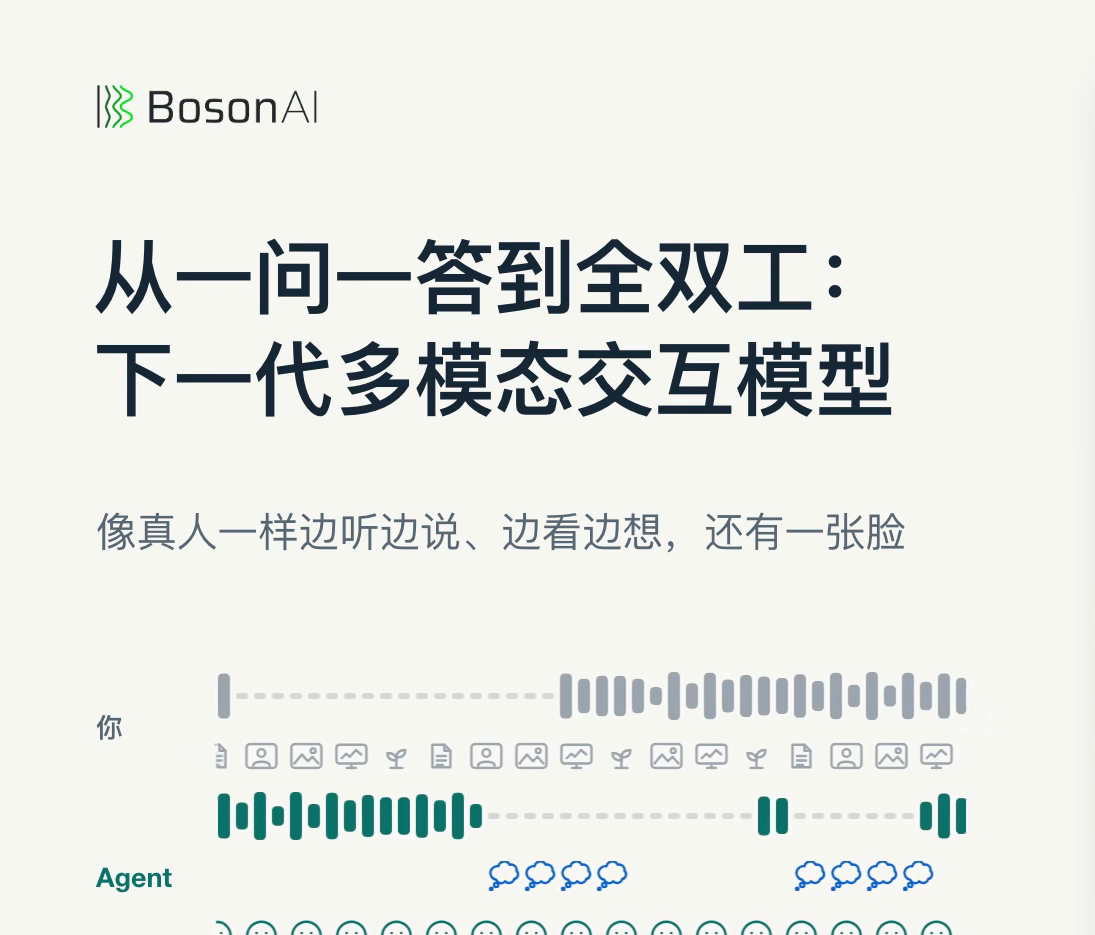
\includegraphics[width=0.76\textwidth]{figures/fig_01_title_slide.png}
\caption{开篇主题：从一问一答到全双工——像真人一样边听边说、边看边想、还拥有一张实时渲染面孔的下一代多模态交互模型\vtag}
\end{figure}
\srcnote{00:00:00--00:00:15}

\begin{enumerate}
    \item \textbf{场景一：团队技术架构会议（Team Meeting）——边看白板、边讲架构、随时响应打断}（图 2）
    在第一个在线会议演示中，Higgs Realtime Duplex 作为会议参与者拥有一张实时渲染的数字人面孔（左上角窗口）。它不仅在共享屏幕（右上角窗口）上向三位人类工程师流利讲解全双工架构图，而且当工程师在中途随时插话提问（如询问它与上一代半双工模型的区别、或要求修改架构图布局）时，模型能在毫秒间立即停下当前话语、听懂问题并结合屏幕上的白板画面实时更新图表。
    \item \textbf{场景二：车载免提与得来速点餐（At the Drive-Thru）——后台查数据 $+$ 自动过滤旁话}（图 3）
    在第二个车载场景中，车主一边开车一边让 Higgs 帮忙查询标普 500 指数（S\&P 500）行情以及后台某项模型训练任务的进度（模型汇报训练已完成约 $68\%$、某项指标稳定在 $94\%$ 左右）。紧接着，车子驶入 In-N-Out 汉堡店的得来速（Drive-Thru）点餐通道，车主转头对着窗口店员点了一份套餐（``just get a double-double meal''）。**此时最惊艳的一幕发生了：模型全程听到了车主与店员的每一句对话，但它精准判断出“这番点餐对话是车主对店员说的，不是对我说的”，因此全程保持安静、绝不乱插嘴！** 等车主点完餐开向取餐窗口并随口问模型“我刚才点动物风味薯条（animal-style fries）了吗？”时，模型立刻回答“没有，你只点了套餐和饮品”——它不仅在后台异步查完了股市和训练任务，还完整记住了刚才的旁话内容！
    \item \textbf{场景三：英语口语私教（Spoken-English Tutor）——看嘴型纠音 $+$ 实时把控练习节奏}（图 4）
    在第三个外语学习场景中，数字人教练先带学习者做 8秒图片限时描述快挑战，随后在发音练习中不仅通过听觉发现学习者把 \texttt{vest}（背心）读成了 \texttt{west}（西方），还通过摄像头实时观察学习者的嘴唇与牙齿咬合动作（要求上牙轻触下唇发 $/v/$ 音），在学习者跟读的瞬间点头附和、纠正口型，交互节奏与真人私教别无二致。
\end{enumerate}

\begin{figure}[H]
\centering
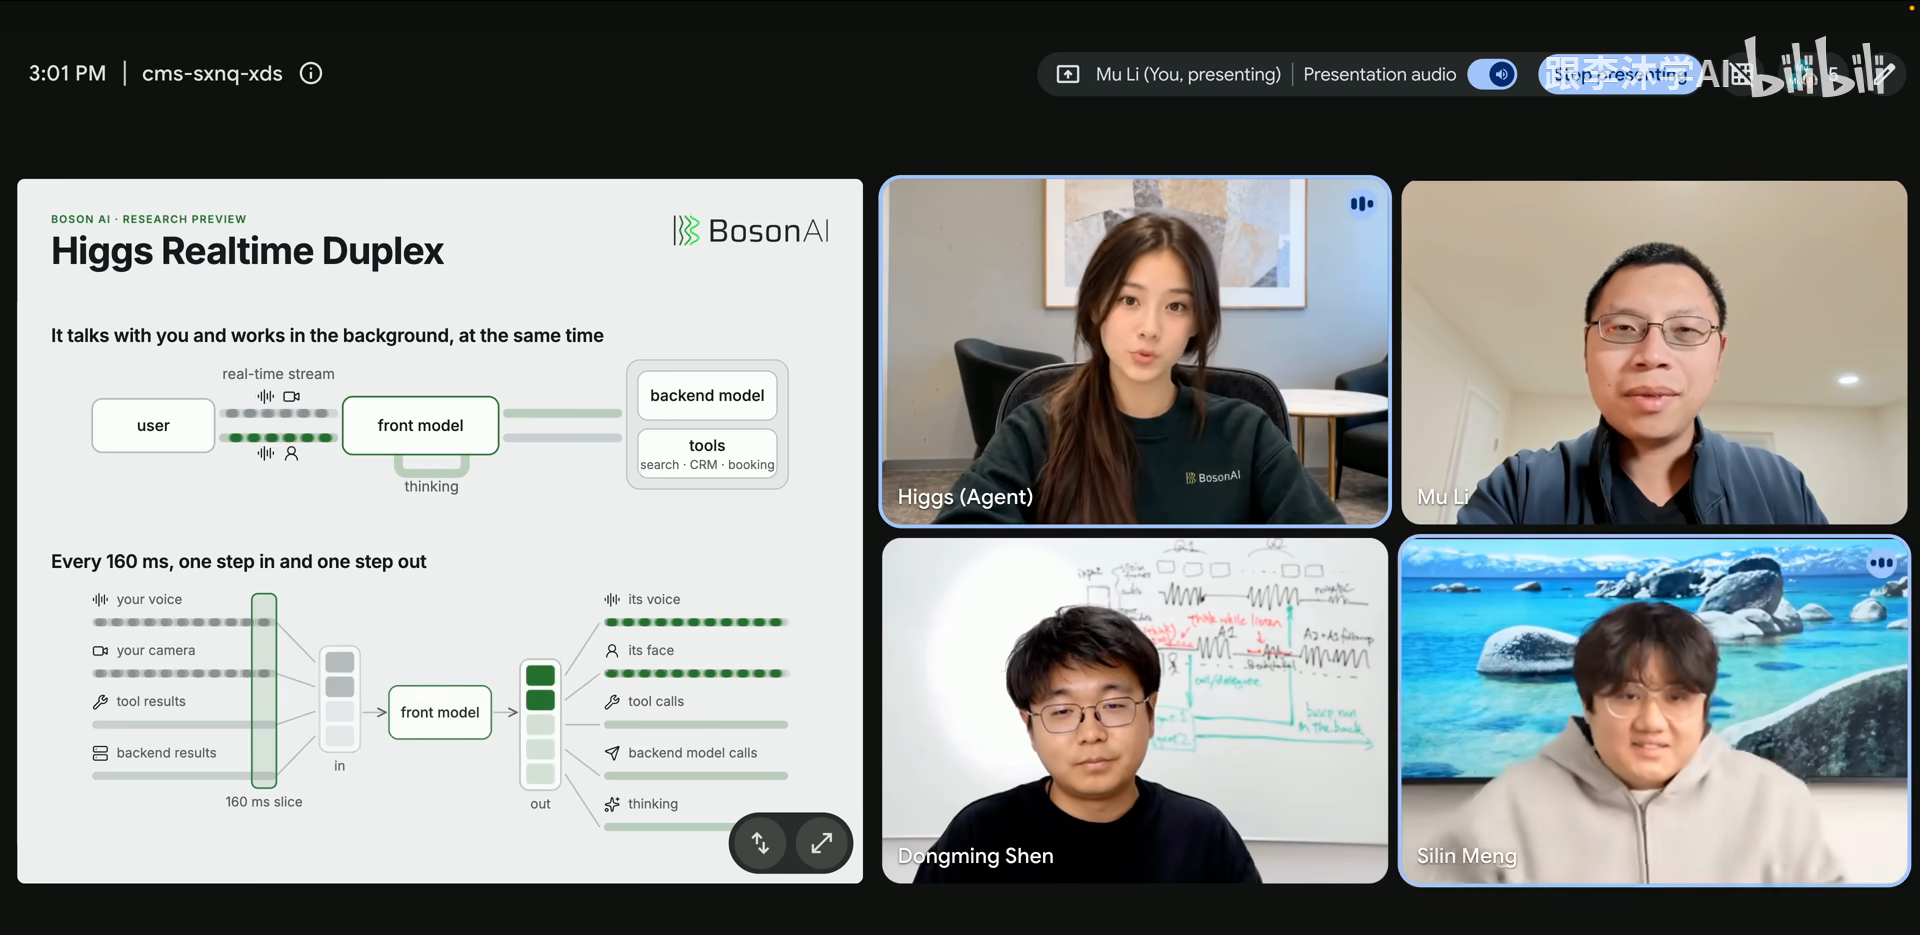
\includegraphics[width=0.92\textwidth]{figures/fig_02_demo_team_meeting.png}
\caption{实机演示一（团队会议）：Higgs Realtime Duplex 实时观察共享屏幕架构图、同步渲染数字人面孔，并自然响应团队成员的中途打断与提问\vtag}
\end{figure}
\srcnote{00:00:30--00:00:45}

\begin{figure}[H]
\centering

\includegraphics[width=0.92\textwidth]{figures/fig_03_demo_drive_thru.png}
\caption{实机演示二（车载 Drive-Thru）：模型在后台异步查询美股行情与训练进度，并在车主向快餐店员点餐时自动识别“非对己旁话”保持安静\vtag}
\end{figure}
\srcnote{00:02:30--00:02:45}

\begin{figure}[H]
\centering
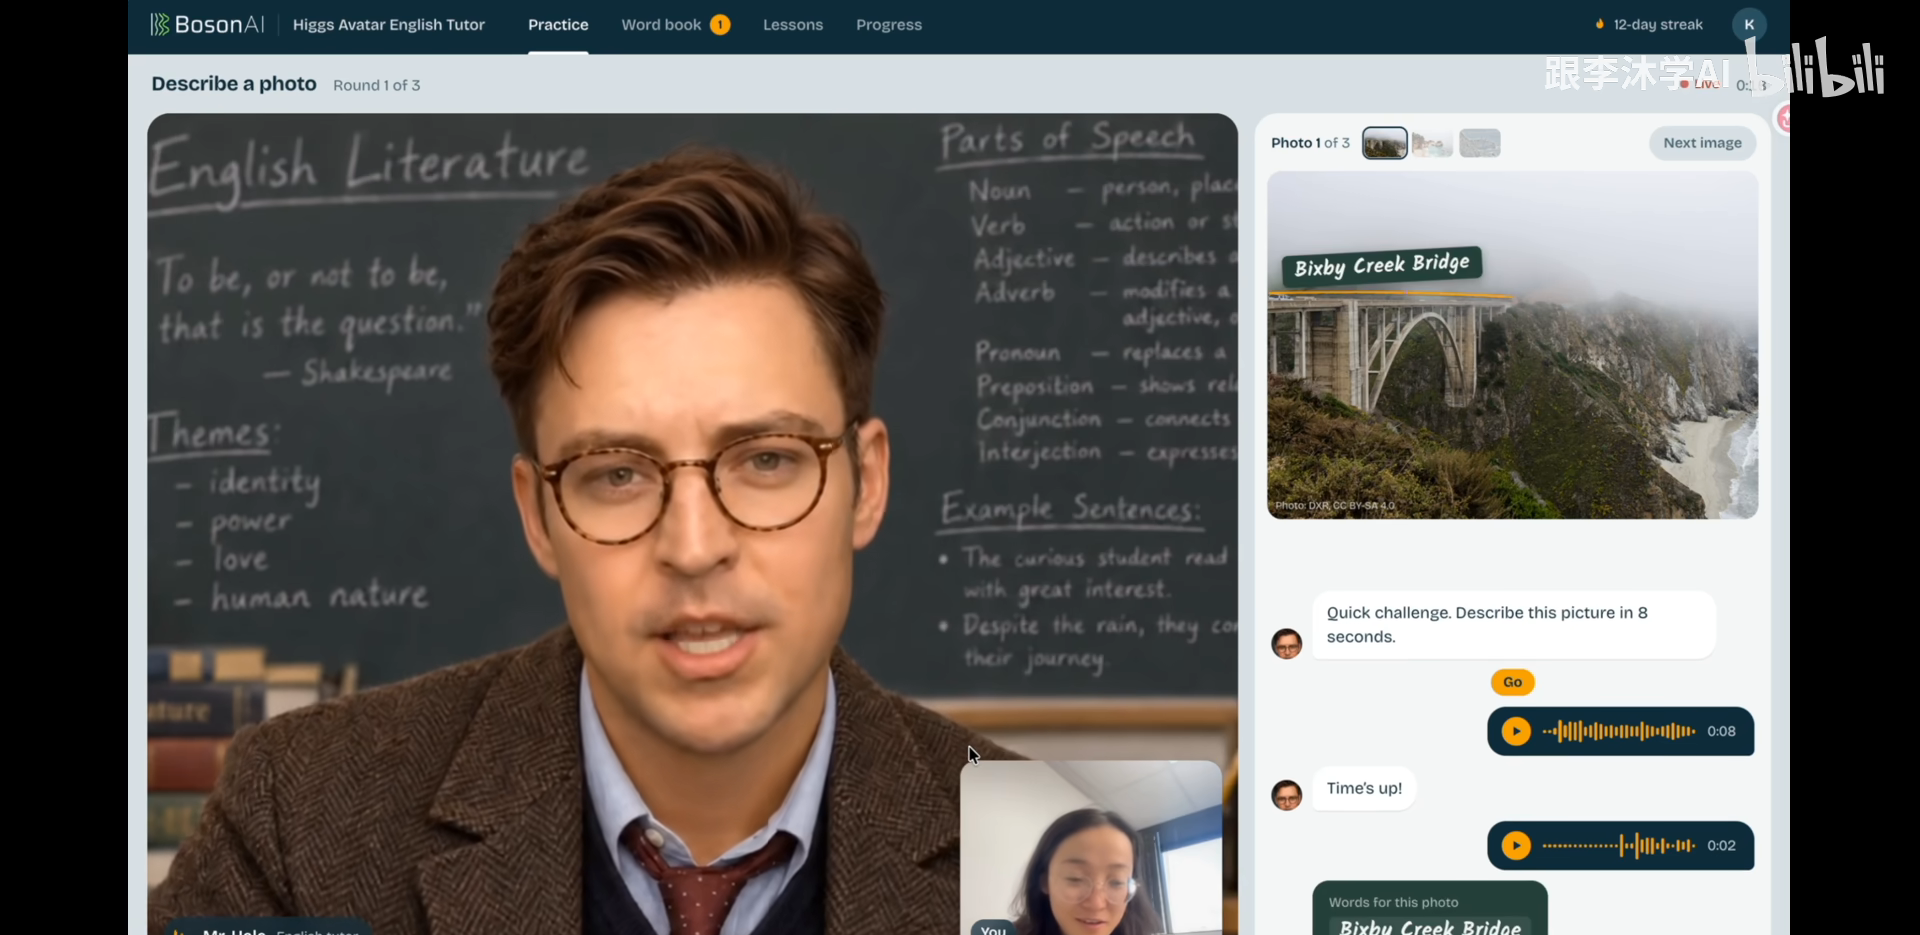
\includegraphics[width=0.92\textwidth]{figures/fig_04_demo_english_tutor.png}
\caption{实机演示三（英语口语私教）：模型通过摄像头实时观察用户嘴型动作，精准纠正 \texttt{west/vest} 发音并把控互动练习节奏\vtag}
\end{figure}
\srcnote{00:04:15--00:04:30}

\subsection{什么样的交互模型才算好？——“像人、够聪明、成本低”黄金三角}

看完三个演示后，李沐老师提出了构建下一代交互模型的第一性原理问题：**如果我们要做一个让用户每天愿意跟它聊好几个小时的交互模型，它到底需要同时满足哪三个核心条件？**（图 5、图 6、图 7）

\begin{figure}[H]
\centering
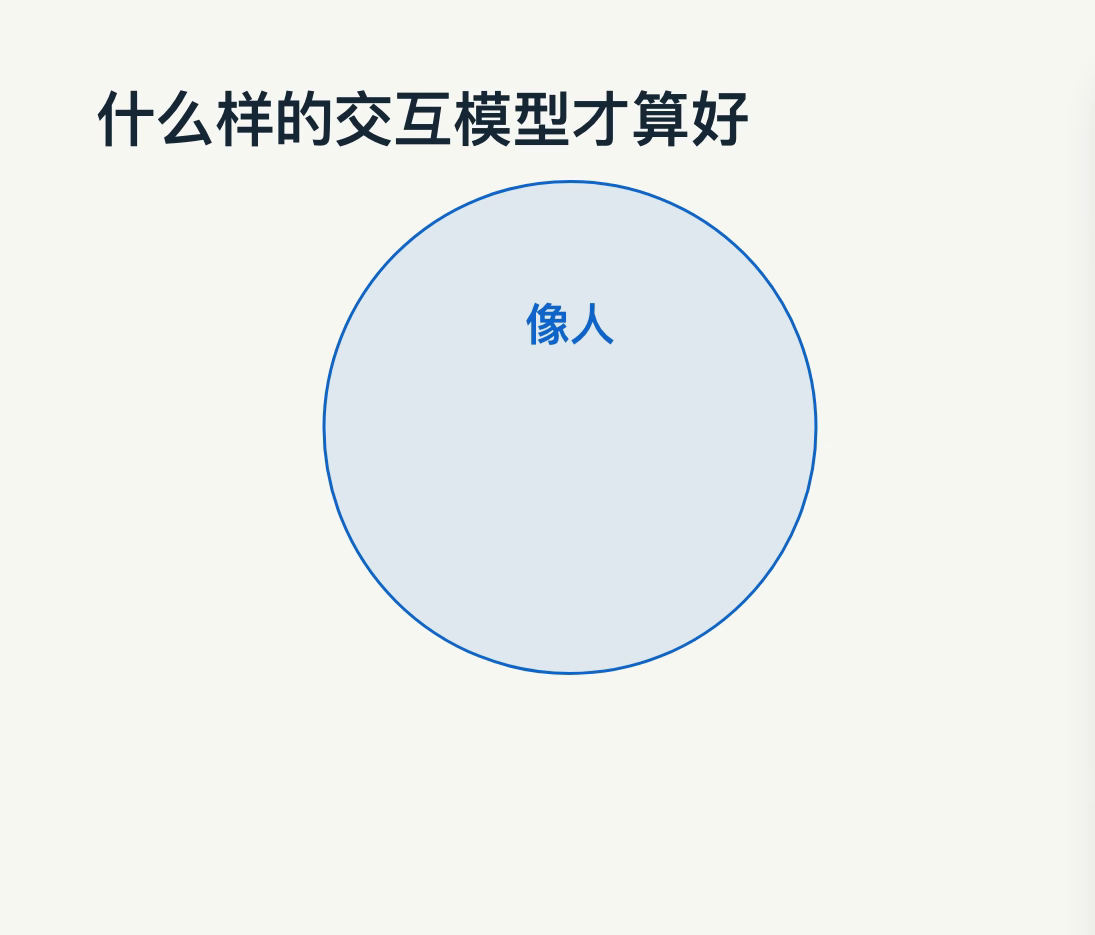
\includegraphics[width=0.72\textwidth]{figures/fig_05_good_model_human_like.png}
\caption{好交互模型的第一维度（像人）：200毫秒以内极速响应、实时倾听附和与打断、非目标旁话静默，以及视觉可见的数字人表情\vtag}
\end{figure}
\srcnote{00:06:00--00:06:15}

\newpage
\begin{figure}[H]
\centering
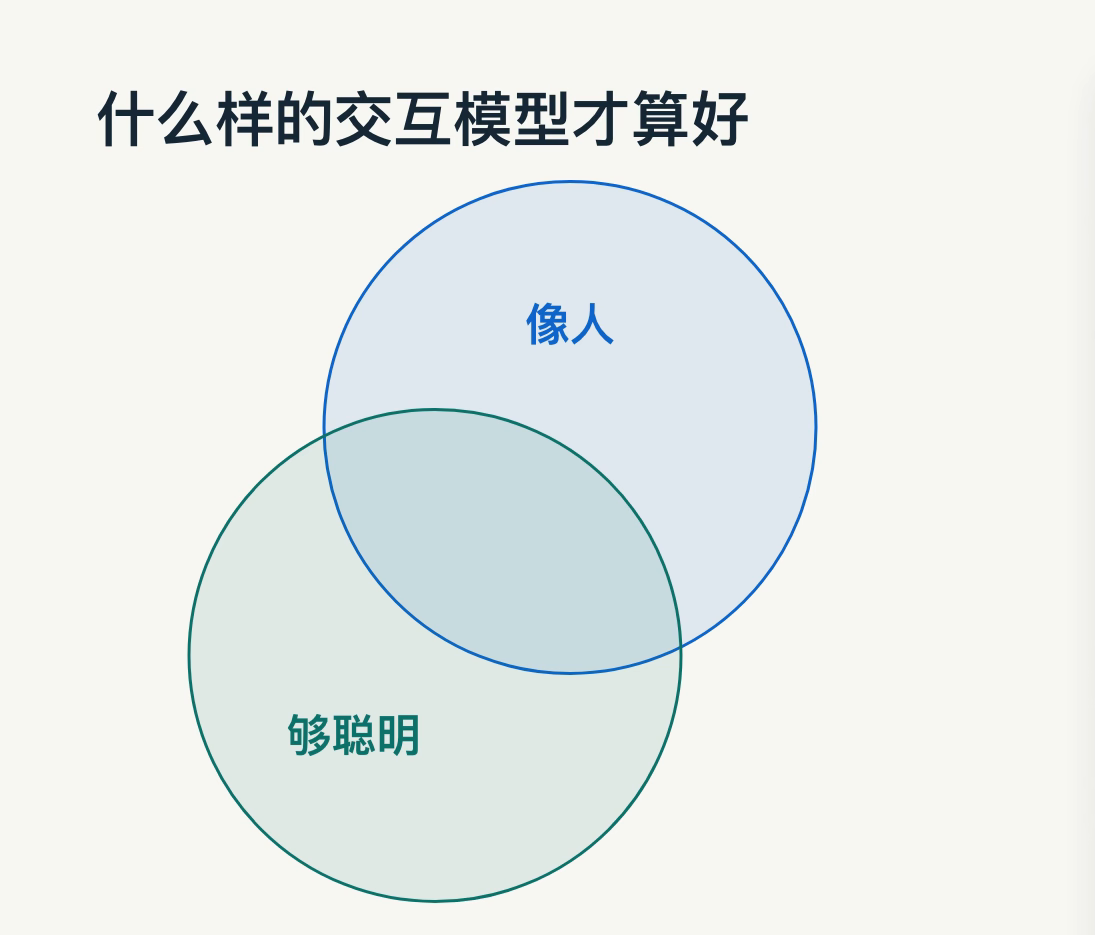
\includegraphics[width=0.66\textwidth]{figures/fig_06_good_model_smart.png}
\caption{好交互模型的第二维度（够聪明）：既要有读懂语气与场景的“情商”，又要有拆解模糊任务、调用工具解决实际问题的“智商”\vtag}
\end{figure}
\srcnote{00:07:30--00:07:45}

\begin{figure}[H]
\centering
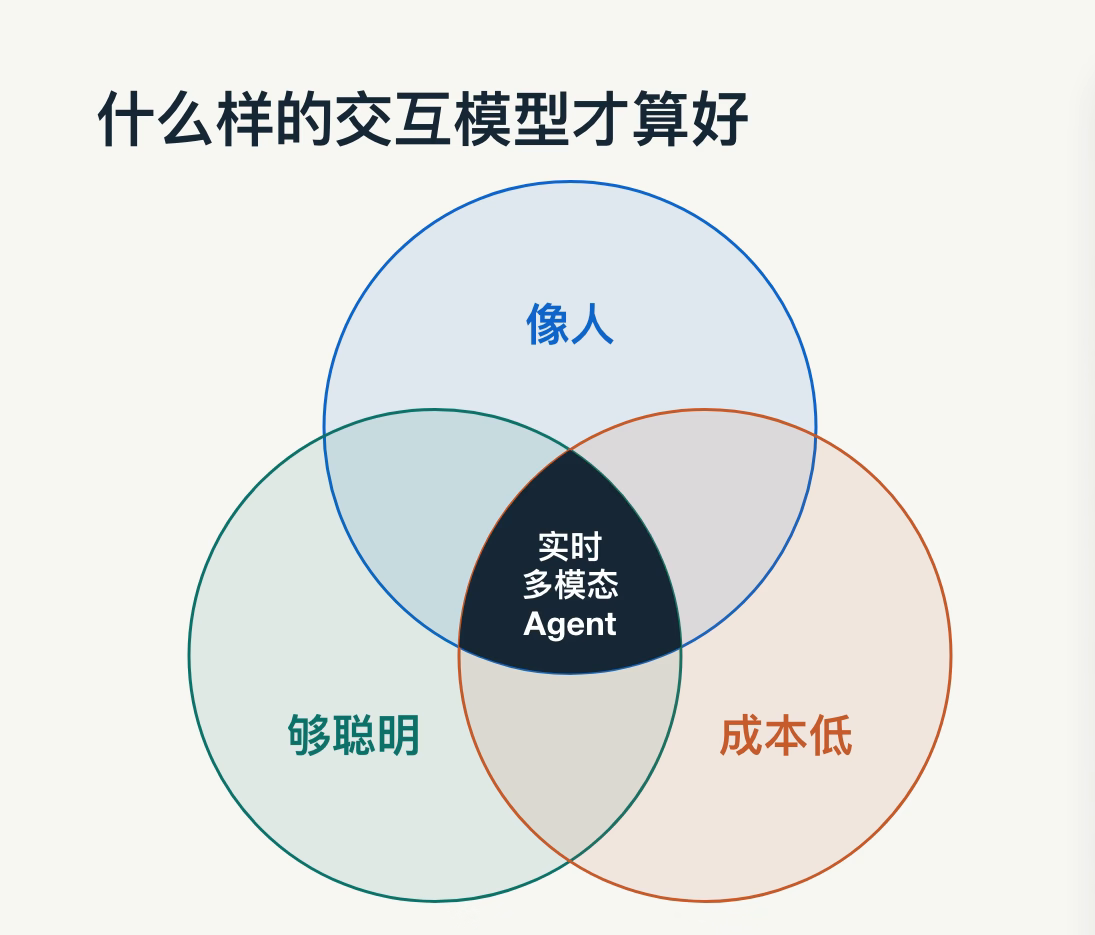
\includegraphics[width=0.66\textwidth]{figures/fig_07_good_model_venn_three.png}
\caption{好交互模型的黄金三角交集：同时满足“像人（Feels Human）”、“够聪明（Smart）”与“成本低（Costs Little）”才能成为日常普及的多模态 Agent\vtag}
\end{figure}
\srcnote{00:09:45--00:10:00}

我们将这三大维度的工程指标形式化为如下联合设计目标：

\begin{equation}
\mathcal{G}_{\mathrm{duplex}}
= \underbrace{\big(T_{\mathrm{resp}} \le 200\,\mathrm{ms},\;\text{Full-Duplex}\big)}_{\text{1. 像人 (Feels Human)}}
\;\cap\;
\underbrace{\big(\mathrm{EQ} + \mathrm{IQ}_{\mathrm{agent}}\big)}_{\text{2. 够聪明 (Smart)}}
\;\cap\;
\underbrace{\Big(C_{\mathrm{model}} \le \frac{1}{10}\,C_{\mathrm{human}}\Big)}_{\text{3. 成本低 (Costs Little)}}
\end{equation}

上式中三个维度的具体内涵如下：
\begin{enumerate}
    \item \textbf{像人（Feels Human）——自然的时间节奏与多模态双向感知}：
    在真实人类对话中，当一方话音刚落，另一方的回应通常在 **200毫秒以内** 就会响起；有时甚至在对方还没说完最后两个字但语义已明朗时，回应就已经自然接上了。更重要的是，真人绝不是木头桩子：你在说话时，对方会边听边点头、发出“嗯哼（mm-hm）”的倾听反馈（Backchanneling）；当你卡壳忘词时对方会主动帮腔；当你中途插话打断时对方会立刻闭嘴让出话轮；而当你转头跟旁边的第三人说话（或背景有电视声、嘈杂噪音）时，对方知道这话不是对自己说的，会安静旁听而不乱接话。此外，面对面交流时人类还会通过眼神、表情与手势传递信息，因此模型不仅要“能看（看摄像头与屏幕）”，最好自己也“有一张能实时做出丰富表情的脸”。
    \item \textbf{够聪明（Smart）——高情商（EQ）与高智商（IQ）缺一不可}：
    如果一个模型只是反应快、声音像人，但聊两句就答非所问、干不了正事，用户新鲜感过去后很快就会抛弃它。真正能帮用户把事情办成的模型，一方面需要**高情商（Emotional Intelligence）**，能够从用户的语气、停顿和面部神态中读出言外之意与当前情境；另一方面需要**高智商（Reasoning \& Agency）**，能够把用户口头随口交代的模糊指令拆解为结构化步骤，在后台主动搜索资料、读写 CRM/日历、运行代码工具并完成复杂任务。
    \item \textbf{成本低（Costs Little）——每小时运行成本不超过人工时薪的 $1/10$}：
    李沐老师预判，未来不善打字或追求高效的普通人与 AI 协作的主要方式就是全天候语音视频交互，每天连接时长可达数小时。如果请一位真人助理或家教一小时需要数十美元，那么 AI 交互模型的设计目标必须是**每小时综合推理成本至多只有真人一小时成本的十分之一（$\le 1/10$）**。只有把成本压到这个量级，全双工多模态 Agent 才能真正走进千家万户。
\end{enumerate}

\begin{importantbox}{核心判断：为什么“三圆交集”极其苛刻？}
在现有技术体系下，这三个目标天然互相拉扯：要想“像人（$\le 200\,\mathrm{ms}$ 低延迟）”，模型就不能太大、不能慢吞吞地做长思维链；要想“够聪明”，又需要大模型级别的推理与长工具调用链；要想“全双工随时看视频听声音”，每秒钟涌入的海量音视频 Token 又会让推理成本指数级爆炸。后续三大架构的演进，本质上就是为了破解这一不可能三角！
\end{importantbox}

\subsection{本章小结}

本章通过团队架构会议、车载点餐与英语口语私教三个实机演示，确立了下一代多模态交互模型的黄金三角标准：像人（200毫秒内响应、全双工倾听附和与打断、数字人视觉形象）、够聪明（情商 $+$ 智商工具调用）与成本低（不超过人工时薪的 $1/10$）。

% =========================================================================
% SECTION 2
% =========================================================================
\section{第一代架构：经典分段式流水线（ASR $+$ LLM $+$ TTS）及其致命缺点}

\subsection{经典分段式架构（Cascaded Pipeline）与语义 VAD 改进}

为了理解为什么要做全双工架构，我们先剖析目前工业界应用最广泛的**第一代架构——经典分段式架构（Cascaded / Modular Pipeline）**（图 8）。

\begin{figure}[H]
\centering
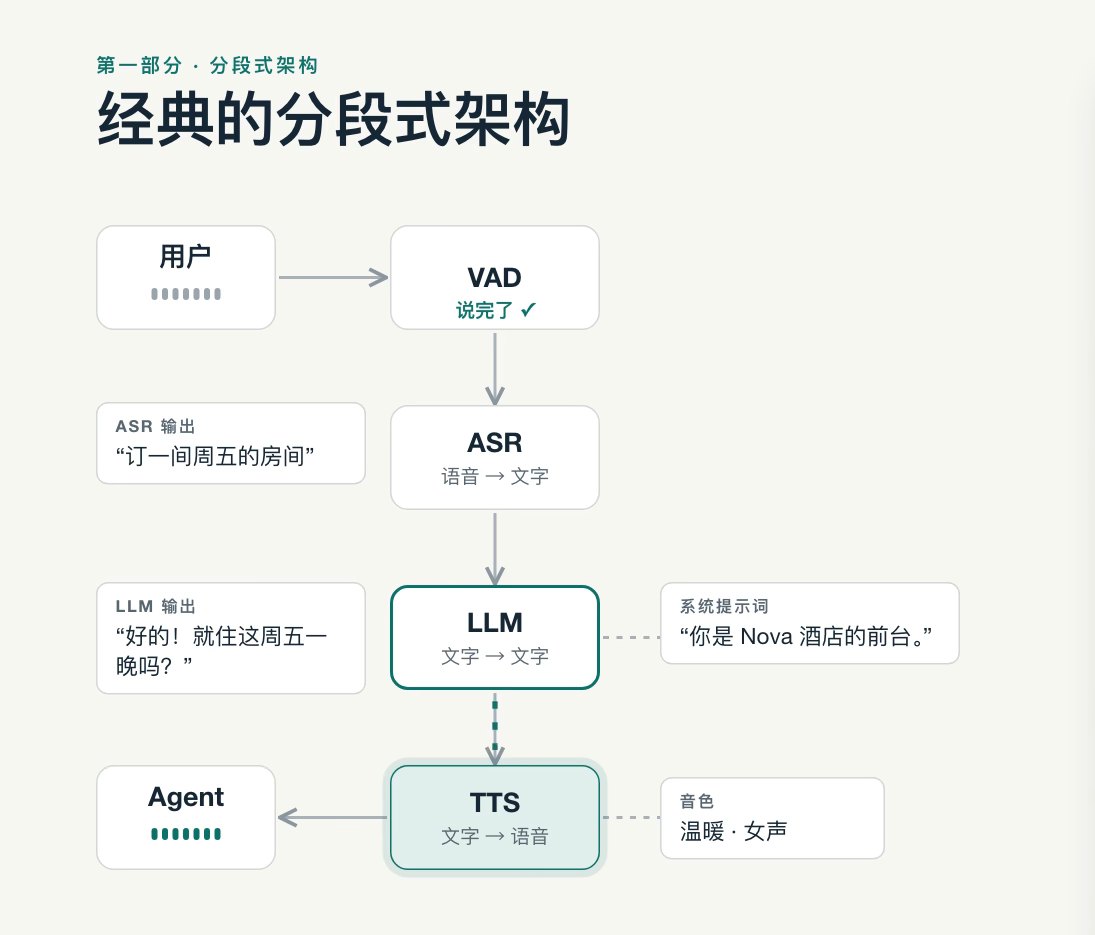
\includegraphics[width=0.74\textwidth]{figures/fig_08_cascaded_pipeline_arch.png}
\caption{经典的分段式架构：由 VAD（语音活动检测）、ASR（语音转文字）、LLM/Agent（文本推理与工具调用）和 TTS（文字转语音）四个独立模块串行拼接而成\vtag}
\end{figure}
\srcnote{00:11:00--00:11:15}

在分段式架构中，一次完整的“你说一句、它答一句”严格按以下四步单向流水线推进：
\begin{enumerate}
    \item \textbf{VAD（Voice Activity Detection，语音活动检测）}：一个极轻量的声学小模型实时监听麦克风音频流。当检测到人声时开始录音缓存；当检测到用户停止说话、连续静音达到预设阈值（例如等 300毫秒、500毫秒，或者保守一点等 1.5秒）时，判定“用户这句话说完了”，将该段音频切出并送往下游。
    \item \textbf{ASR（Automatic Speech Recognition，自动语音识别）}：将切出的用户语音片段转录为纯文本字符串（例如 \texttt{"帮我查一下明天的天气"}）。
    \item \textbf{LLM $+$ Agent（大语言模型与智能体工具调用）}：接收 ASR 转写出的纯文本，结合历史上下文进行文本推理，必要时调用外部搜索或业务 API，生成回复文本。
    \item \textbf{TTS（Text-to-Speech，语音合成）}：将 LLM 生成的回复文本合成为音频波形播放给用户；若在播放途中 VAD 又检测到用户开口说话，则强行清空当前播放队列实现打断。
\end{enumerate}

在早期实践中，工程师很快发现**纯声学 VAD 存在一个极其尴尬的阈值两难困境**（图 9）：人类说话在句中思考或换气时，常常会有几百毫秒的自然停顿。如果你把 VAD 静音阈值设得很短（比如 300毫秒或 400毫秒），用户刚说出“我今天早上去了……”喘口气的功夫，VAD 就误以为用户说完了，直接把半截话切给 LLM 抢话回答；反之，如果你为了防止抢话把阈值拉长到 1秒甚至 1.5秒，那么当用户干脆利落地问完一句“今天几号？”后，系统也必须傻等 1.5秒才开始转写，交互体验变得极其迟钝。

\begin{figure}[H]
\centering
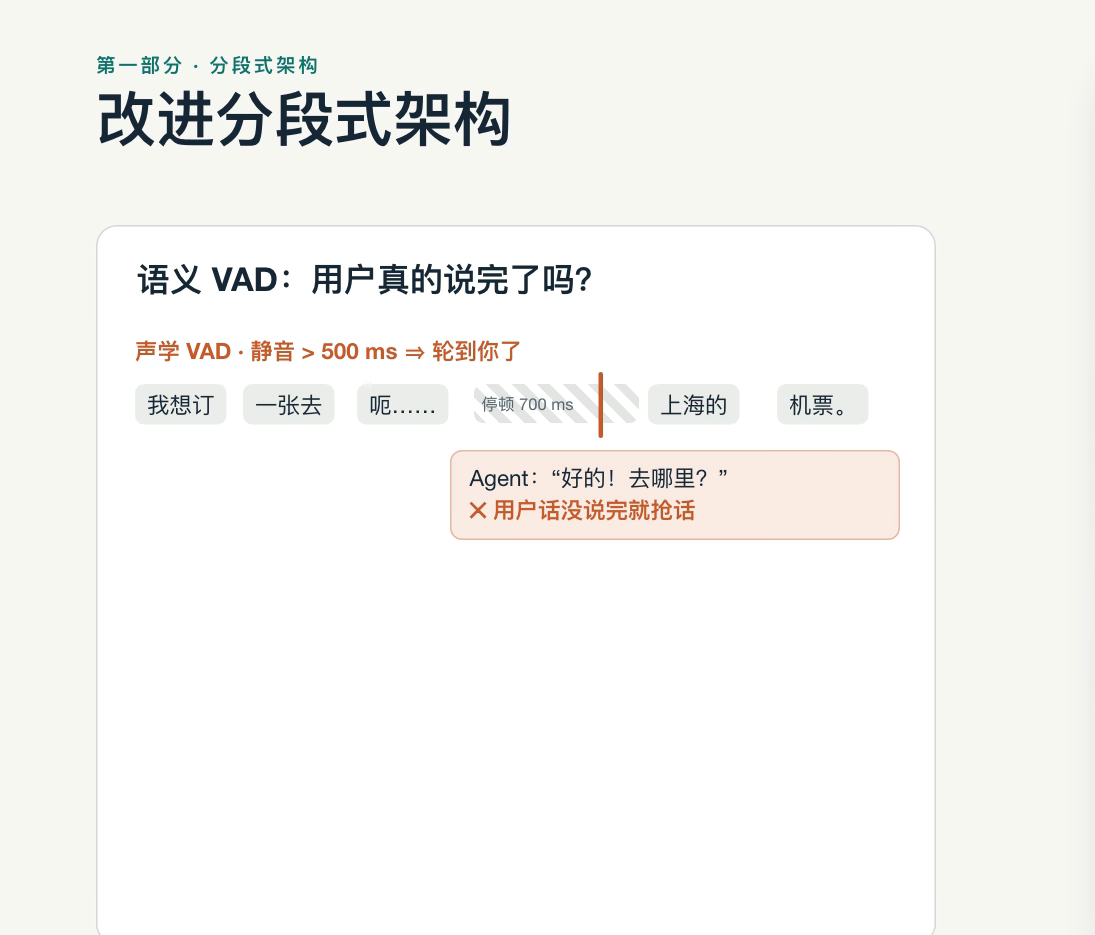
\includegraphics[width=0.74\textwidth]{figures/fig_09_semantic_vad_upgrade.png}
\caption{改进分段式架构（一）：引入语义 VAD（Semantic VAD），结合声学静音检测（如 400毫秒）与语义完整性判断用户是否真正把话说完\vtag}
\end{figure}
\srcnote{00:12:15--00:12:30}

\begin{figure}[H]
\centering
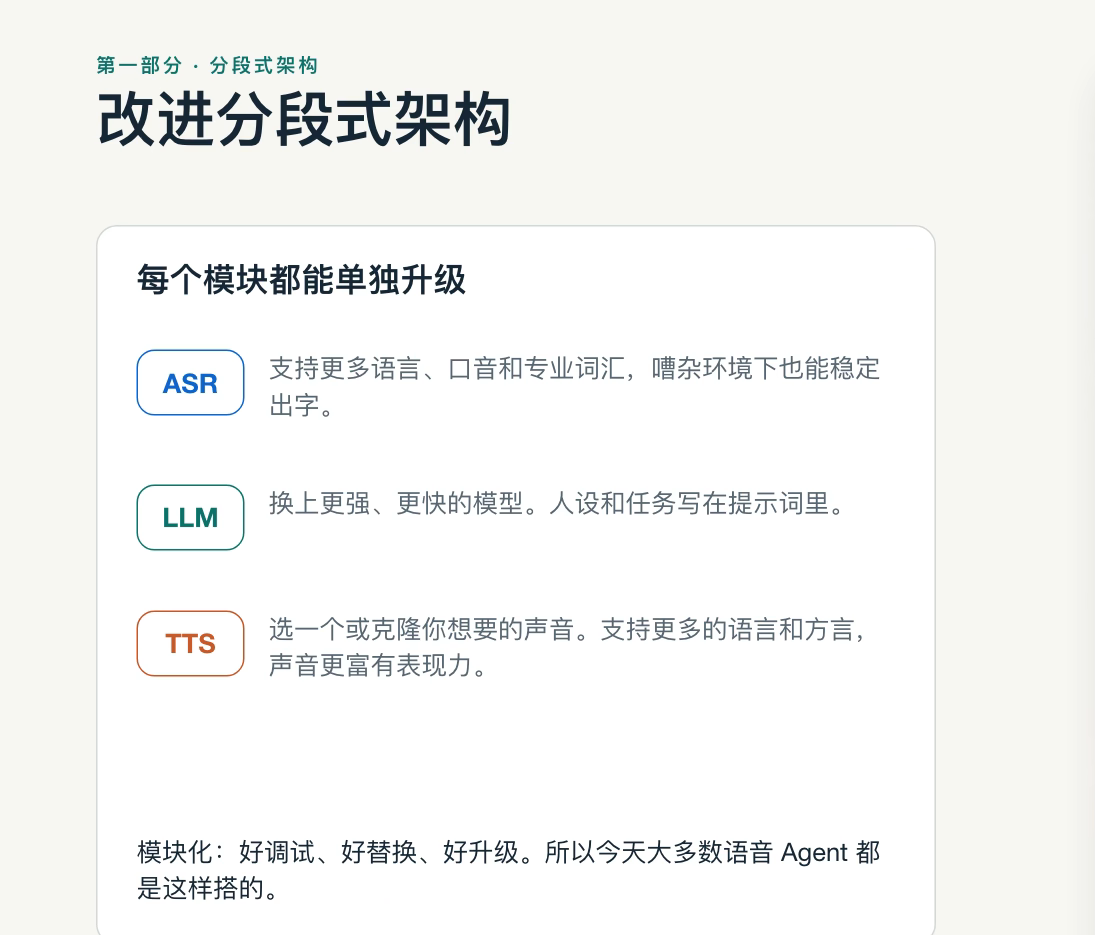
\includegraphics[width=0.74\textwidth]{figures/fig_10_modular_independent_upgrade.png}
\caption{改进分段式架构（二）：模块化解耦使得 ASR、LLM 与 TTS 可以由不同团队独立升级替换，因此成为当前市面上绝大多数语音 Agent 的首选架构\vtag}
\end{figure}
\srcnote{00:13:15--00:13:30}

为此，现代改进版分段式架构普遍引入了**语义 VAD（Semantic VAD）**（图 9）：当声学 VAD 检测到约 400毫秒静音时，先结合流式 ASR 已转写出的文字看一眼语义是否完整——如果文字是“那今天天气怎么样”（语义已完整，标点结句），就立即触发回复；如果文字是“我今天早上去了……”（明显的半截话），就继续耐心等待用户把后半句说完。

同时，分段式架构拥有一个巨大的工程落地优势（图 10）：**模块彻底解耦，每个模块都能单独升级**。你可以直接拿开源最好的 Whisper 做 ASR，中间接能力最强的商业闭源文本大模型（如 GPT-4 / Claude）做大脑，最后接效果最好的商业 TTS 做发声。这套组合拳好理解、好调试、好替换，因此直到今天仍是工业界语音 Agent 落地的绝对主力。

\subsection{模块化带来的两个致命缺点：1.7 秒串行延时与“文字细管子”}

既然分段式架构如此成熟，为什么我们不能一直沿着这条路修修补补走下去？李沐老师犀利地指出了模块化流水线无法克服的**两个致命结构性缺陷**（图 11、图 12）：

\begin{figure}[H]
\centering
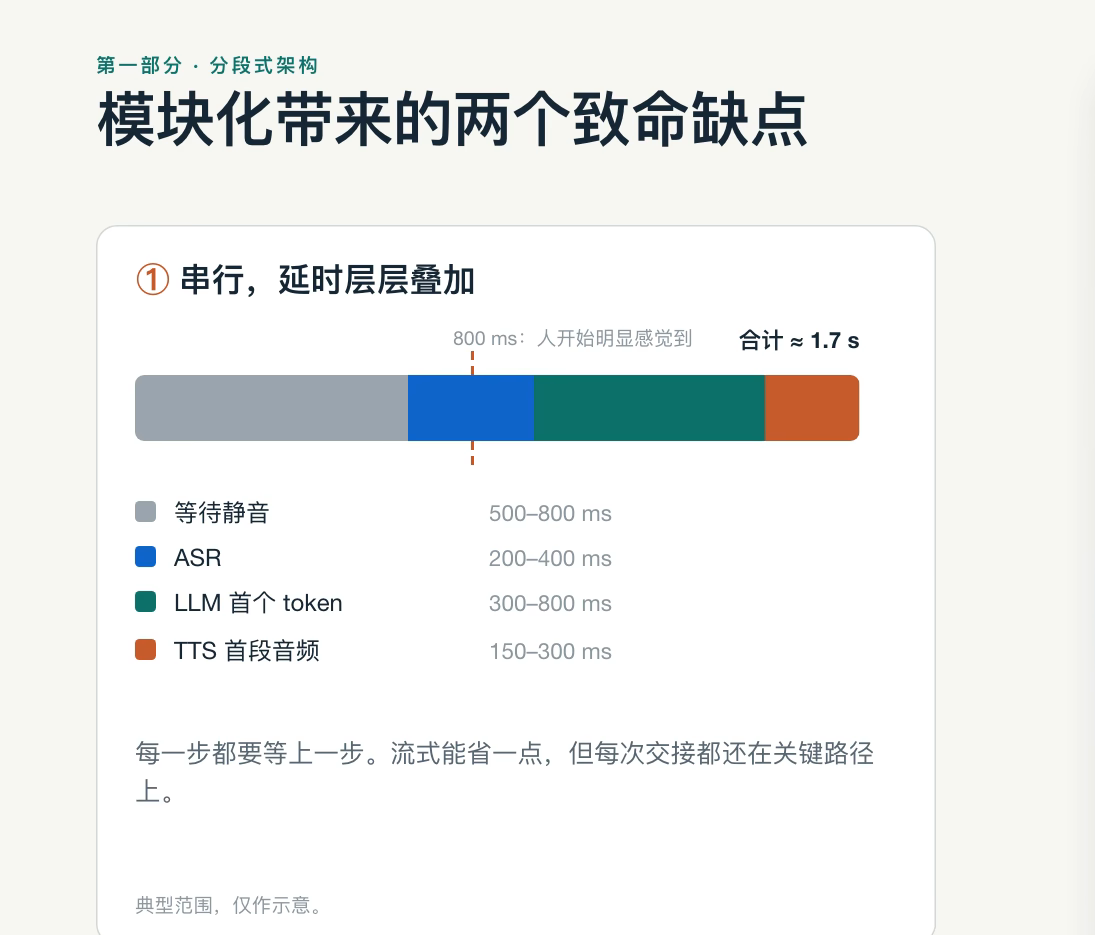
\includegraphics[width=0.66\textwidth]{figures/fig_11_cascaded_latency_stack.png}
\caption{模块化带来的致命缺点（一）：串行流水线导致延时层层叠加，合计响应延迟高达约 $1.7\,\mathrm{s}$（1.5秒到 2秒），远超人类开始明显感到卡顿的 800毫秒阈值\vtag}
\end{figure}
\srcnote{00:14:15--00:14:30}

\begin{figure}[H]
\centering
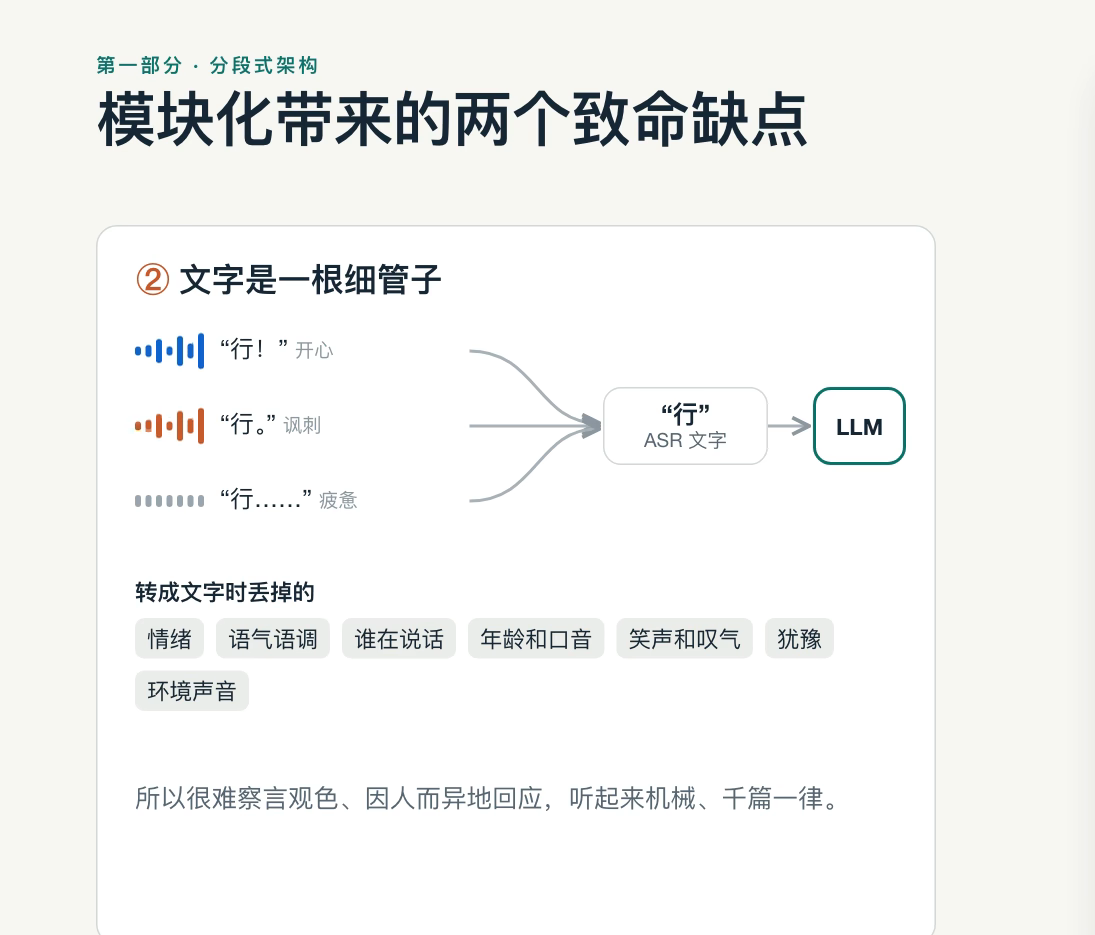
\includegraphics[width=0.66\textwidth]{figures/fig_12_text_narrow_pipe_bottleneck.png}
\caption{模块化带来的致命缺点（二）：“文字是一根细管子”——丰富的副语言声学特征在 ASR 端被全部丢弃，TTS 只能靠干瘪文字盲猜语气，导致语音机械千篇一律\vtag}
\end{figure}
\srcnote{00:16:00--00:16:15}

\subsubsection{致命缺点一：串行流水线，延时层层叠加（$\approx 1.7\,\mathrm{s}$）}
在分段式架构中，四个模块在关键路径上串联交接，即便采用流式（Streaming）传输能省掉一部分尾部等待，首包响应延迟 $T_{\mathrm{cascaded}}$ 依然是四段刚性开销的线性加和：

\begin{equation}
T_{\mathrm{cascaded}}
= \underbrace{T_{\mathrm{VAD\_silence}}}_{500\text{--}800\,\mathrm{ms}}
+ \underbrace{T_{\mathrm{ASR}}}_{200\text{--}400\,\mathrm{ms}}
+ \underbrace{T_{\mathrm{LLM\_TTFT}}}_{300\text{--}800\,\mathrm{ms}}
+ \underbrace{T_{\mathrm{TTS\_first}}}_{150\text{--}300\,\mathrm{ms}}
\;\approx\; 1.15\text{--}2.30\,\mathrm{s} \quad (\text{典型值 } \approx 1.7\,\mathrm{s})
\end{equation}

上式中各分项的实测耗时与人类心理声学阈值的矛盾极为突出：
\begin{itemize}
    \item $T_{\mathrm{VAD\_silence}}$（等待静音确认）：即便有语义 VAD 辅助，为了确认用户真的停口，平均仍需等待 $500\text{--}800\,\mathrm{ms}$；
    \item $T_{\mathrm{ASR}}$（语音转写收尾）：将整句音频完成最终对齐并输出确切文本需 $200\text{--}400\,\mathrm{ms}$；
    \item $T_{\mathrm{LLM\_TTFT}}$（大语言模型首 Token 延迟，Time-to-First-Token）：LLM 预填充（Prefill）并蹦出第一个回复词需 $300\text{--}800\,\mathrm{ms}$；
    \item $T_{\mathrm{TTS\_first}}$（TTS 首段音频合成）：TTS 必须攒够头几个词才能确定连读与声调，合成首包音频又需 $150\text{--}300\,\mathrm{ms}$。
\end{itemize}
四项加起来，每次用户说完话都要干等 **1.5秒到 2秒（典型值约 $1.7\,\mathrm{s}$）** 才能听到机器开口！而在打电话或面对面交谈时，人类对 **800毫秒到 1秒以上** 的停顿是极其敏感的——一旦超过 800毫秒对方还没出声，你就会明显感觉到尴尬的冷场（Dead Air），甚至怀疑电话是不是掉线了。

\subsubsection{致命缺点二：“文字是一根细管子”（信息论瓶颈）}
第二个致命缺点在于模块之间的接口形态：**ASR、LLM 与 TTS 之间仅靠纯文本字符串（Text）通信，而“文字是一根极细的管子”**（图 12）！

从信息论视角看，一段真实的人类语音信号 $X_{\mathrm{audio}}$ 蕴含的信息远不止字面词汇 $W_{\mathrm{text}}$，还包含极其丰富的副语言与环境特征 $Z_{\mathrm{para}}$（说话人的年龄、性别、语速快慢、重音位置、叹气、笑声、哽咽、迟疑、反讽语调以及背景环境音）。当 ASR 强行将语音投影到纯文本空间时，发生了不可逆的信息坍缩：

\begin{equation}
I(X_{\mathrm{audio}}; Y_{\mathrm{LLM}})
\le H(W_{\mathrm{text}})
\ll H(W_{\mathrm{text}}, Z_{\mathrm{para}}) = H(X_{\mathrm{audio}})
\end{equation}

其中 $I(\cdot\,;\,\cdot)$ 表示互信息，$H(\cdot)$ 表示信息熵。举例来说，同样一句文字 \texttt{"行吧，都听你的"}：
\begin{itemize}
    \item 如果用户是用轻快愉悦的语调说出来的，代表欣然同意；
    \item 如果用户是先长叹一口气、再用极其委屈低沉或阴阳怪气的语调说出来的，代表强烈的不满与妥协！
\end{itemize}
然而经过 ASR 这根“文字细管子”后，这两种截然相反的情绪变成了冷冰冰的六个相同汉字 \texttt{"行吧，都听你的"}；中间的 LLM 完全听不到那声叹气，只能按字面意思回复；到了下游 TTS 合成时，TTS 也不知道刚才发生了什么上下文，只能用播音员般标准、机械、千篇一律的欢快腔调把回复念出来——即使尝试让 LLM 在文本里加括号标注情绪（如 \texttt{[温柔地]}），由于这种情绪标签极其稀疏粗糙，依然无法还原真实人类语音千变万化的韵律表现力。

\begin{warningbox}{架构警示：为什么修补分段式流水线无法通向终极交互？}
只要架构中间还隔着“必须先把连续语音切成段 $\to$ 转成纯文本字符串 $\to$ 再把文本转回语音”这道强制序列化关卡，串行延迟下限与副语言信息丢失就是物理学意义上的死结。要打破这道墙，必须拆开 ASR 与 TTS 的黑盒！
\end{warningbox}

\subsection{本章小结}

本章剖析了由 `VAD -> ASR -> LLM -> TTS` 组成的第一代分段式架构及其语义 VAD 改进，揭示了其难以逾越的两大瓶颈：四阶段串行叠加导致的高达约 $1.7\,\mathrm{s}$ 的响应延迟（远超 800毫秒人类感知阈值），以及纯文本接口作为“细管子”造成的副语言情绪与环境信息丢失。

% =========================================================================
% SECTION 3
% =========================================================================
\section{第二代架构：端到端多模态模型（End-to-End）与遗留的三大痛点}

\subsection{拆开 ASR 与 TTS 看看：从三个 Decoder 合一到端到端音视频模型}

既然“文字细管子”和“多模块交接”是罪魁祸首，我们能不能把 ASR、LLM 和 TTS 融合成同一个模型？为了看清这件事为什么可行，李沐老师首先带我们拆开了现代神经网络 ASR（以 Whisper 为代表）与现代神经 TTS 的内部黑盒（图 13、图 14）：

\begin{figure}[H]
\centering
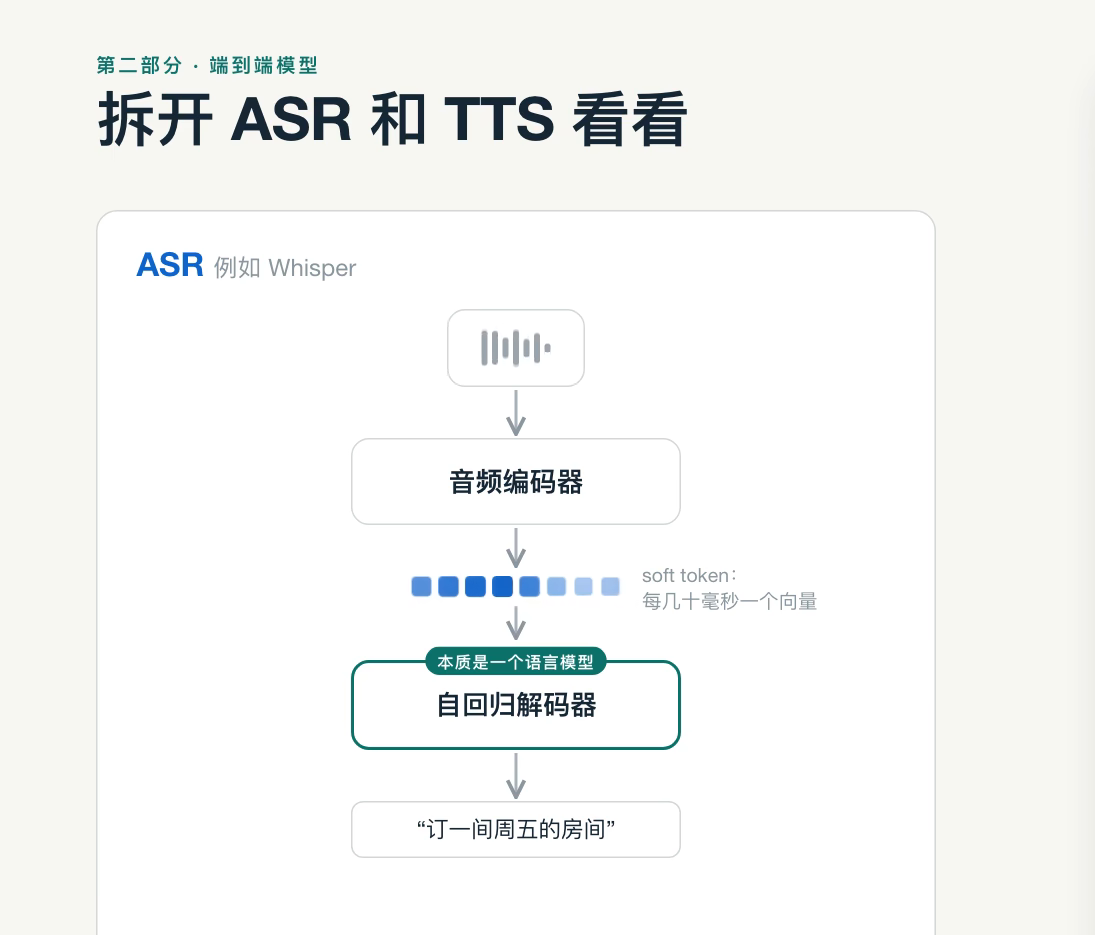
\includegraphics[width=0.74\textwidth]{figures/fig_13_inside_asr_and_tts.png}
\caption{拆开 ASR 与 TTS 内部结构：现代 ASR（音频编码器 $+$ 文本解码器）与现代自回归 TTS（语音生成模型 $+$ Codec 音频解码器）均以 Transformer 为核心组件\vtag}
\end{figure}
\srcnote{00:17:15--00:17:30}

\begin{figure}[H]
\centering
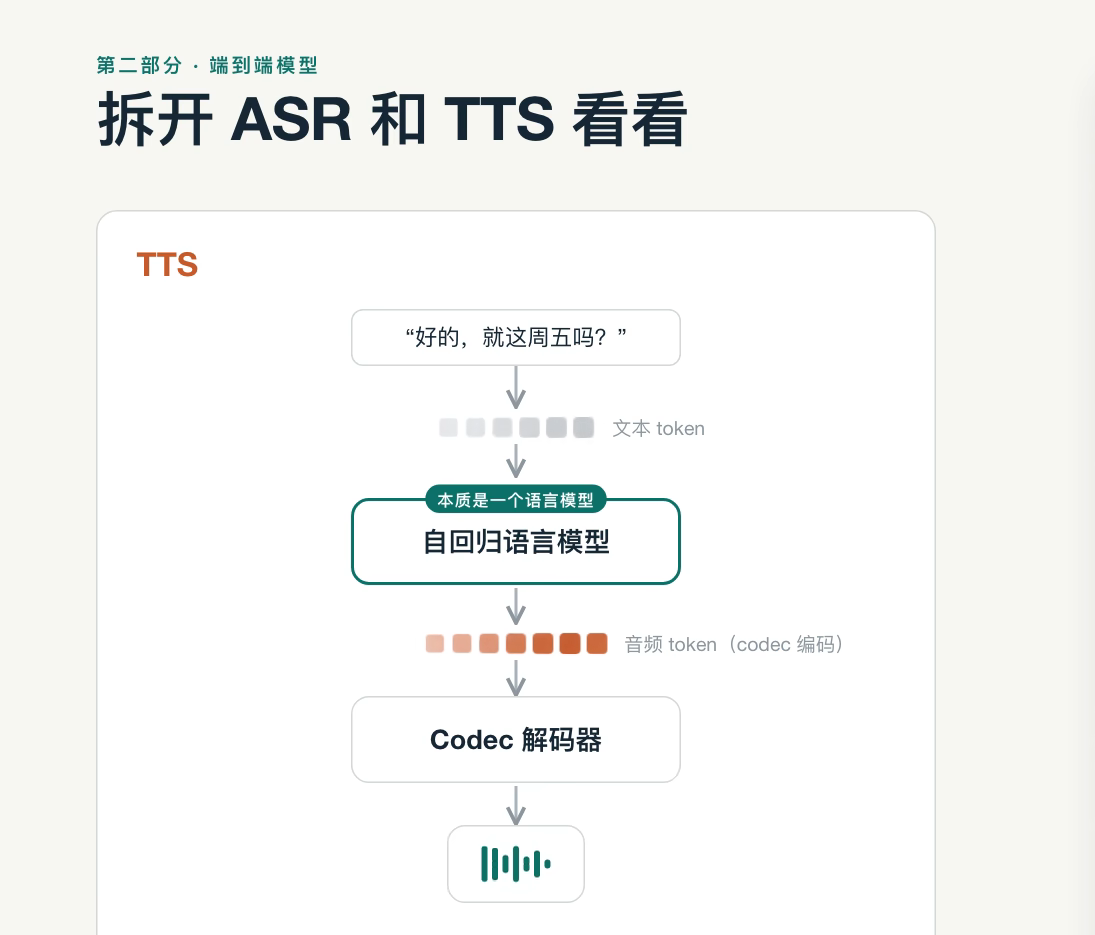
\includegraphics[width=0.74\textwidth]{figures/fig_14_merge_three_decoders.png}
\caption{合成一个模型（一）：由于 ASR 解码器、LLM 主干与 TTS 自回归生成器本质上全都是 Decoder-only Transformer，完全可以将三者合并为单一多模态骨干网络\vtag}
\end{figure}
\srcnote{00:18:45--00:19:00}

请仔细观察图 13 与图 14 的结构对应关系：
\begin{enumerate}
    \item \textbf{现代 ASR（如 OpenAI Whisper）是怎么工作的？}
    输入的连续语音波形首先按固定时间窗（例如每 **80毫秒** 切成一个片段）送入一个**音频编码器（Audio Encoder）**，直接转化成一串连续的高维特征向量（Embedding）；随后通过一个基于 Transformer 的**文本解码器（Decoder）**，把这串音频特征向量一个词一个词地解码成文字 Token。
    \item \textbf{现代神经 TTS 是怎么工作的？}
    它接收文字 Token（以及一段用于指定音色的参考语音 Embedding），通过一个**自回归语音语言模型（Autoregressive Speech Model，本质上也是一个 Decoder-only Transformer）**，一步步预测出代表声音声学特征的离散或连续**音频 Token（Audio Tokens）**；最后再由一个轻量的**音频 Codec 解码器（Audio Decoder）**把音频 Token 还原成可播放的声波。
    \item \textbf{三合一的惊人洞察}：
    把 ASR、LLM、TTS 摆在一起（图 14），你会惊讶地发现：**ASR 的后半截（文本 Decoder）、中间的 LLM（文本 Decoder-only Transformer）以及 TTS 的前半截（自回归语音 Decoder），在数学结构上全都是一模一样的自回归 Transformer 解码器！** 既然如此，为什么要让三个 Transformer 用文字接力传话，而不直接把它们合并成**同一个多模态大语言模型（Multimodal LLM）**呢？
\end{enumerate}

合三为一之后，我们就得到了**第二代架构——端到端多模态语音/音视频架构（End-to-End Architecture）**（图 15、图 16）：

\begin{figure}[H]
\centering
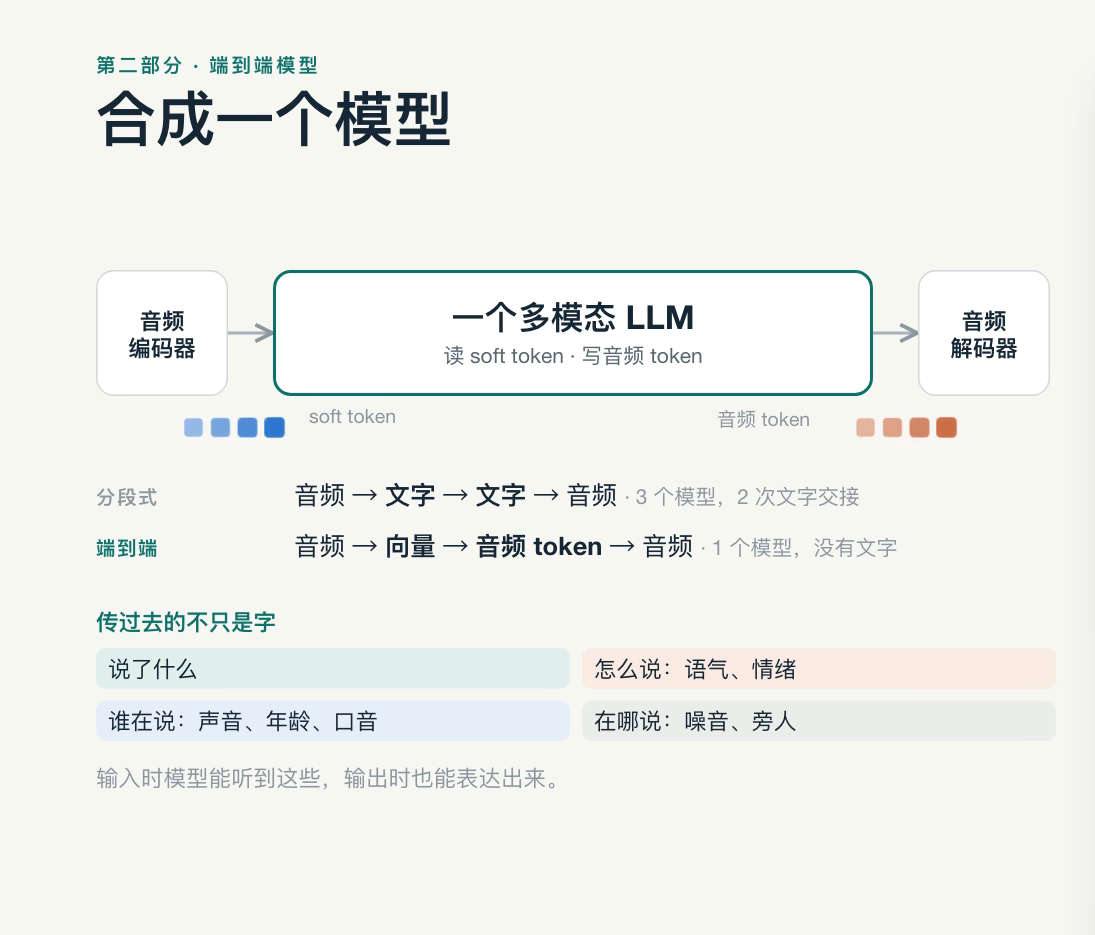
\includegraphics[width=0.66\textwidth]{figures/fig_15_unified_multimodal_llm.png}
\caption{合成一个模型（二）：单一多模态 LLM 直接吃进音频编码器输出的连续声学向量，并在内部同时生成文本 Token 与富有表现力的音频 Token\vtag}
\end{figure}
\srcnote{00:21:00--00:21:15}

\begin{figure}[H]
\centering
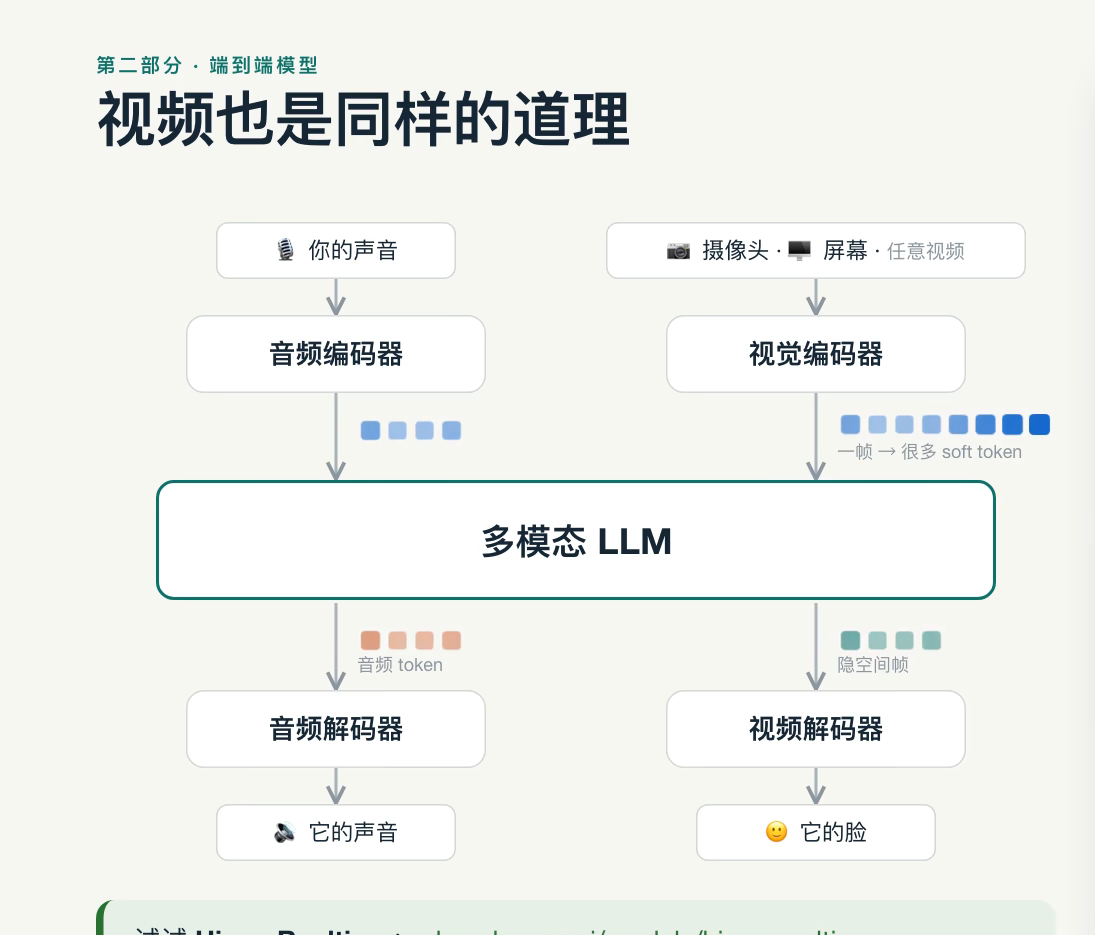
\includegraphics[width=0.66\textwidth]{figures/fig_16_end_to_end_audio_video.png}
\caption{视频也是同样的道理：在端到端语音架构上进一步接入视频编码器与数字人视频解码器，构成支持音视频输入输出的 \texttt{Higgs Realtime} 端到端模型\vtag}
\end{figure}
\srcnote{00:23:15--00:23:30}

\begin{knowledgebox}{第二代架构剖析：端到端多模态 LLM 是如何同时解决延时与表现力的？}
在图 15 与图 16 所示的端到端模型（即 Boson AI 已上线的 \texttt{Higgs Realtime}）中：
\begin{enumerate}
    \item \textbf{彻底消灭“文字细管子”}：用户的原始语音经轻量级音频编码器提取为高维声学 Embedding 后，直接送入多模态 LLM 的注意力层。模型不仅能“听清”用户说了什么字，还能在隐空间（Latent Space）中直接感知用户的语调、年龄、情绪起伏与环境背景音；输出时，LLM 直接自回归地吐出包含丰富情感与重音韵律的音频 Token，交给末端 Codec 解码器流式发声，语音自然度发生质的飞跃。
    \item \textbf{保留文本与音频交织生成（Interleaved Text \& Audio）}：为了让模型不丢失在海量纯文本上习得的高智商，端到端模型在输出音频 Token 的同时也会同步输出对应的内部文本 Token（或先蹦出文本 Token 紧跟着蹦出对应的音频 Token），使语言智商与语音表现力在同一个主干网络中无缝对齐。
    \item \textbf{自然扩展至视觉输入与数字人视频输出}（图 16）：与音频完全同构，只需在输入端挂接一个**视频编码器（Video Encoder）**将用户摄像头或屏幕画面转为视觉 Token，在输出端挂接一个**视频解码器（Video Decoder）**将模型输出的视觉隐变量还原为数字人面部视频流，即可实现端到端音视频交互。
    \item \textbf{端到端延时减半（压缩至 0.7到0.9秒）}：省去了独立 ASR 转写完毕与独立 TTS 攒词预热的中间环节后，当 VAD 判定用户说完话时，音频特征已在模型上下文中就绪，模型立刻吐出首个音频 Token 发声。加上公网传输开销，实测端到端响应延迟通常在 **0.7到0.9秒** 之间，相比分段式架构（$1.5\text{--}2.0\,\mathrm{s}$）快了一倍以上！
\end{enumerate}
\end{knowledgebox}

\subsection{端到端架构仍有三个问题没解决：VAD 矛盾、轮次锁定与工具阻塞}

既然端到端架构已经把延迟压到了 0.7秒左右，且声音富有感情，为什么我们还需要再往前迈一步做“全双工”？李沐老师在幻灯片第 9 页（图 17）中深刻指出了端到端半双工架构依然无法克服的**三大遗留顽疾**：

\begin{figure}[H]
\centering
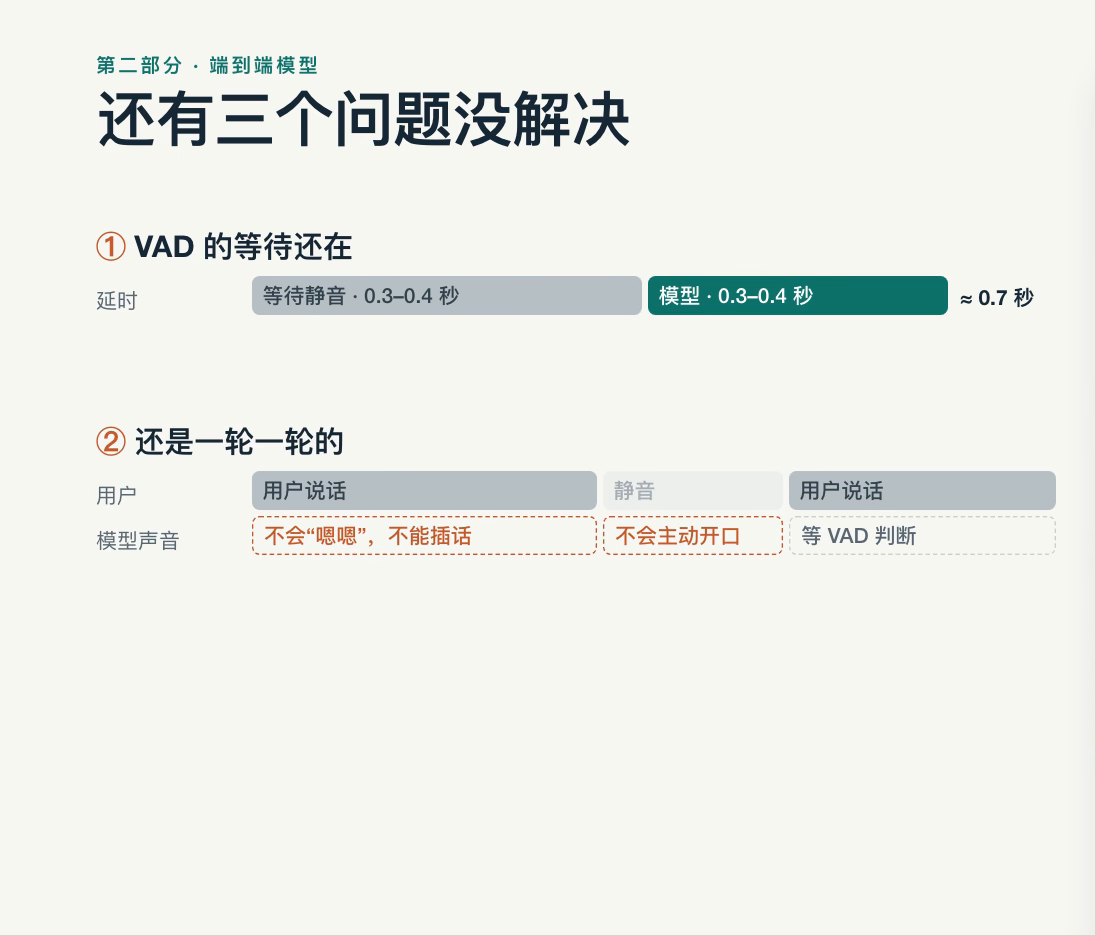
\includegraphics[width=0.74\textwidth]{figures/fig_17_three_unsolved_problems.png}
\caption{端到端架构仍有三个核心问题没解决：(1) VAD 的根本矛盾（快慢两难）、(2) 依然是一轮一轮的半双工交互、(3) 工具调用会卡住当前轮次\vtag}
\end{figure}
\srcnote{00:25:15--00:25:30}

\begin{enumerate}
    \item \textbf{问题一：VAD 的根本矛盾（快慢两难）依然存在}
    哪怕模型本身生成首包只需 0.3秒，只要外层还套着一个“等用户说完再触发模型”的 VAD 开关，你就永远逃不出 VAD 的宿命：比如端到端链路本身已有 0.7秒延时，如果你要求 VAD 检测到 **0.34秒** 的静音就立刻触发模型回复，那么总延时虽然压到了 1秒左右，但用户说话中途稍微喘口气（停顿 0.34秒）就会被模型粗暴打断抢话；反之，如果把 VAD 调慢，总延迟又会退化回 1.5秒以上。更何况，外置的小型 VAD 模型根本不具备主模型的深层多模态上下文，无法准确分辨“用户是在对我说话，还是在跟旁边的店员点餐”。
    \item \textbf{问题二：依然是“一轮一轮”的半双工（Turn-based），无法边听边说}
    在端到端半双工模型中，状态机在任意时刻只能处于“纯倾听（Prefill 输入）”或“纯说话（Decode 输出）”二选一的互斥状态。当用户在长篇大论倾诉时，模型就像木头一样完全沉默，无法像真人那样每隔几秒轻轻回应一声“嗯嗯”、“对，我明白”来提供情绪价值与倾听确认；而当模型在说话时，除非触发硬打断清空整个回合，否则它也无法根据用户微小的表情变化或插话实时调整自己正在说的内容。
    \item \textbf{问题三：思考与工具调用会彻底“卡死”当前轮次（Blocking Tool Calls）}
    这是制约端到端语音模型智商上限最致命的枷锁！因为用户对语音响应延迟极其敏感（只给你几百毫秒反应时间），模型收到语音后必须立刻开口说话，**根本没有时间先做几秒钟的深度思维链（Chain-of-Thought）推理**；更糟糕的是，一旦模型决定调用外部搜索或查询数据库工具，在工具返回结果之前的数秒钟内，整个当前轮次就会陷入死一般的沉默（Dead Air）！为了不冷场，端到端模型往往被迫放弃深度思考与复杂工具调用，导致“语音模型一开口就变笨”。
\end{enumerate}

\subsection{本章小结}

本章通过拆解 Whisper ASR（每 80毫秒音频切片编码）与自回归 TTS 的内部结构，展示了如何将三个 Decoder-only Transformer 合并为单一端到端多模态模型（\texttt{Higgs Realtime}，延时降至 0.7到0.9秒），并指出了半双工范式下仍未解决的三大痛点：VAD 快慢两难（如 0.34秒停顿抢话）、轮次互斥锁定以及思考与工具调用引发的轮次阻塞。

% =========================================================================
% SECTION 4
% =========================================================================
\section{第三代架构：全双工（Full Duplex）——按 160毫秒时间切片而非按轮次}

\subsection{从单线程到多线程：把时间切成固定小片段（Time-Slicing）}

怎样一次性彻底消灭 VAD 矛盾、轮次互斥与工具阻塞这三大顽疾？李沐老师在第三部分给出了全讲最核心的架构跃迁——**抛弃“按说话轮次（Turn）”组织的单线程状态机，改用“按固定时间切片（Time-Slicing）”组织的多线程全双工流式架构**（图 18）！

\begin{figure}[H]
\centering
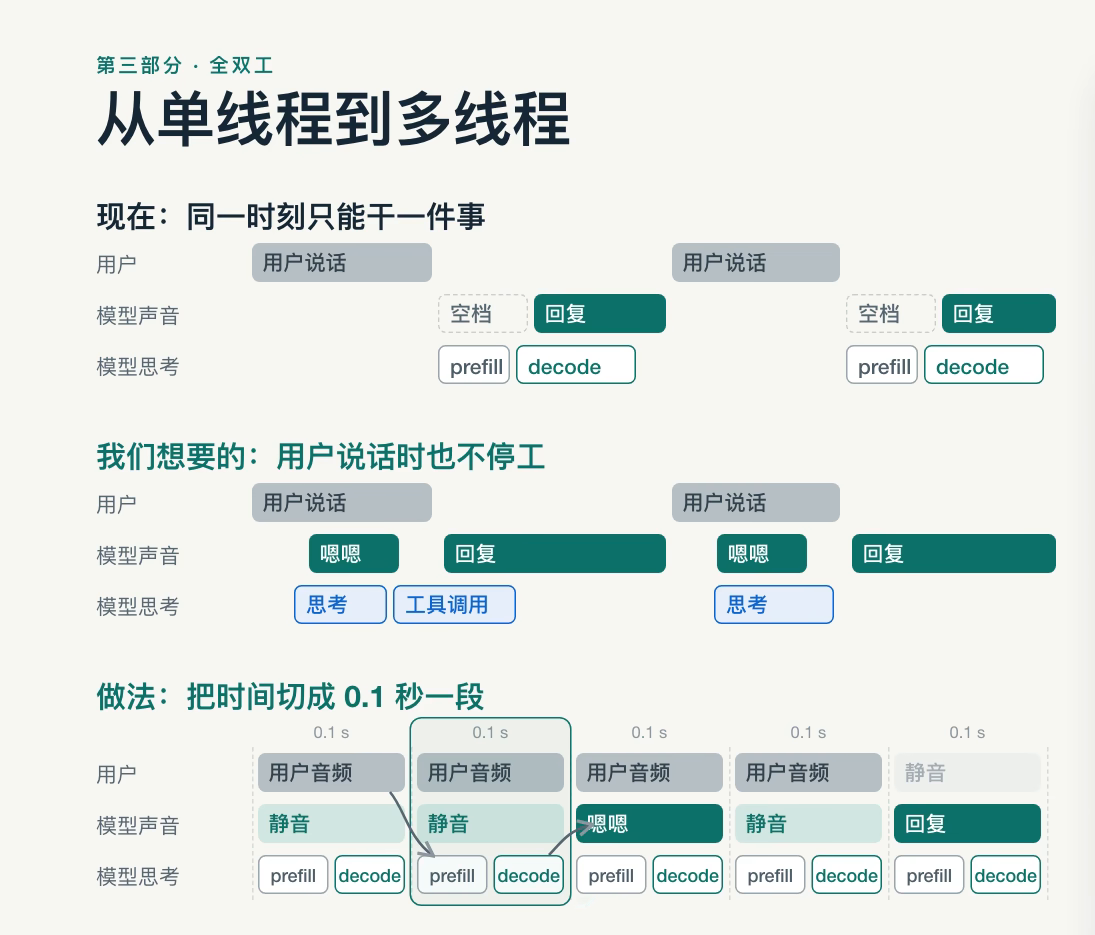
\includegraphics[width=0.74\textwidth]{figures/fig_18_single_to_multi_thread.png}
\caption{从单线程到多线程：打破“用户说一轮 $\to$ 模型答一轮”的串行等待，将连续时间切分为 0.1秒（实际工程取 160毫秒）一段的微观时间片，在每个时间片内同时处理听说与后台思考\vtag}
\end{figure}
\srcnote{00:27:45--00:28:00}

让我们先跟随图 18 的直观推导理解这一范式转换：
\begin{itemize}
    \item \textbf{过去的单线程模式（上）}：同一时间只能干一件事。用户说话时模型只做输入编码；等 VAD 判定用户闭嘴后，模型才开始思考、调工具、再输出语音。
    \item \textbf{我们想要的多线程全双工模式（中）}：用户在说话的同时，模型不仅在听、在看，还在后台同步做思考（Thinking）和工具调用（Tool Calling），甚至根据需要同时发出“嗯哼”的附和声——用户说话时模型绝不闲着，模型干活时也绝不停止倾听！
    \item \textbf{具体工程做法——按时间切片（下）}：为了在单个自回归 Transformer 主干上实现这种并发流，我们将连续的物理时间轴切分为固定长度 $\Delta \tau$ 的小时间窗（课堂概念推导时先以 $\Delta \tau = 0.1\text{秒}$ 为例，而在 \texttt{Higgs Realtime Duplex} 实际工程中精确设定为 **$\Delta \tau = 160\text{毫秒} = 0.16\text{秒}$**，即每秒钟固定推进 $6.25$ 步）。
\end{itemize}

在每一个 $\Delta \tau = 160\text{毫秒}$ 的时间步 $t$ 内，模型严格执行一次“读入当前输入块 $\mathcal{X}_t \to$ 预测下一输出块 $\mathcal{Y}_t$”的因果状态转移：

\begin{equation}
\mathcal{Y}_t
= \Big\langle y_t^{\mathrm{audio}},\; y_t^{\mathrm{face}},\; y_t^{\mathrm{think}},\; y_t^{\mathrm{tool/del}} \Big\rangle
= \mathcal{M}_{\mathrm{duplex}}\Big(\mathcal{H}_{<t},\; \underbrace{\big\langle x_t^{\mathrm{audio}},\; x_t^{\mathrm{video}},\; x_t^{\mathrm{ext\_res}} \big\rangle}_{\mathcal{X}_t\;\text{(160 ms Input Chunk)}}\Big)
\end{equation}

上式中各多模态流分量的物理意义如下：
\begin{itemize}
    \item $\mathcal{X}_t = \langle x_t^{\mathrm{audio}}, x_t^{\mathrm{video}}, x_t^{\mathrm{ext\_res}} \rangle$：第 $t$ 个 160毫秒时间片内新到达的**聚合输入块（Input Chunk）**，包含用户在这 160毫秒内的麦克风音频（哪怕用户没说话，静音本身也作为一个静音音频块流入）、摄像头/屏幕画面帧，以及外部工具或后端大模型恰好在该时间片返回的异步结果载荷 $x_t^{\mathrm{ext\_res}}$；
    \item $\mathcal{Y}_t = \langle y_t^{\mathrm{audio}}, y_t^{\mathrm{face}}, y_t^{\mathrm{think}}, y_t^{\mathrm{tool/del}} \rangle$：模型在第 $t$ 步同步生成的、将在下一个 160毫秒时间片播放与执行的**聚合输出块（Output Chunk）**，包含模型自己要发出的语音片段 $y_t^{\mathrm{audio}}$（若模型决定当前时间片保持沉默，则输出静音 Token）、数字人面部表情隐变量 $y_t^{\mathrm{face}}$、内部思维链片段 $y_t^{\mathrm{think}}$ 以及异步工具调用/大模型委派指令片段 $y_t^{\mathrm{tool/del}}$；
    \item $\mathcal{H}_{<t}$：截至 $t-1$ 步的多模态KV Cache 上下文历史。由于每个时间片长度仅为 0.16秒，从用户说完最后一个音节到模型在下一时间片开口发声，理论架构响应延迟直接被压缩到了 **0.1秒至 0.2秒左右**，彻底达到了真人面对面交谈的生理响应极限！
\end{itemize}

\subsection{全双工时序全景与 8 步窗口微观机制剖析}

为了看清这套 160毫秒时间切片机制在真实对话中是如何行云流水般运转的，我们来看幻灯片第 11 页的全景时序图（图 19）及其底部放大后的 8 步微观窗口图（图 20）：

\begin{figure}[H]
\centering
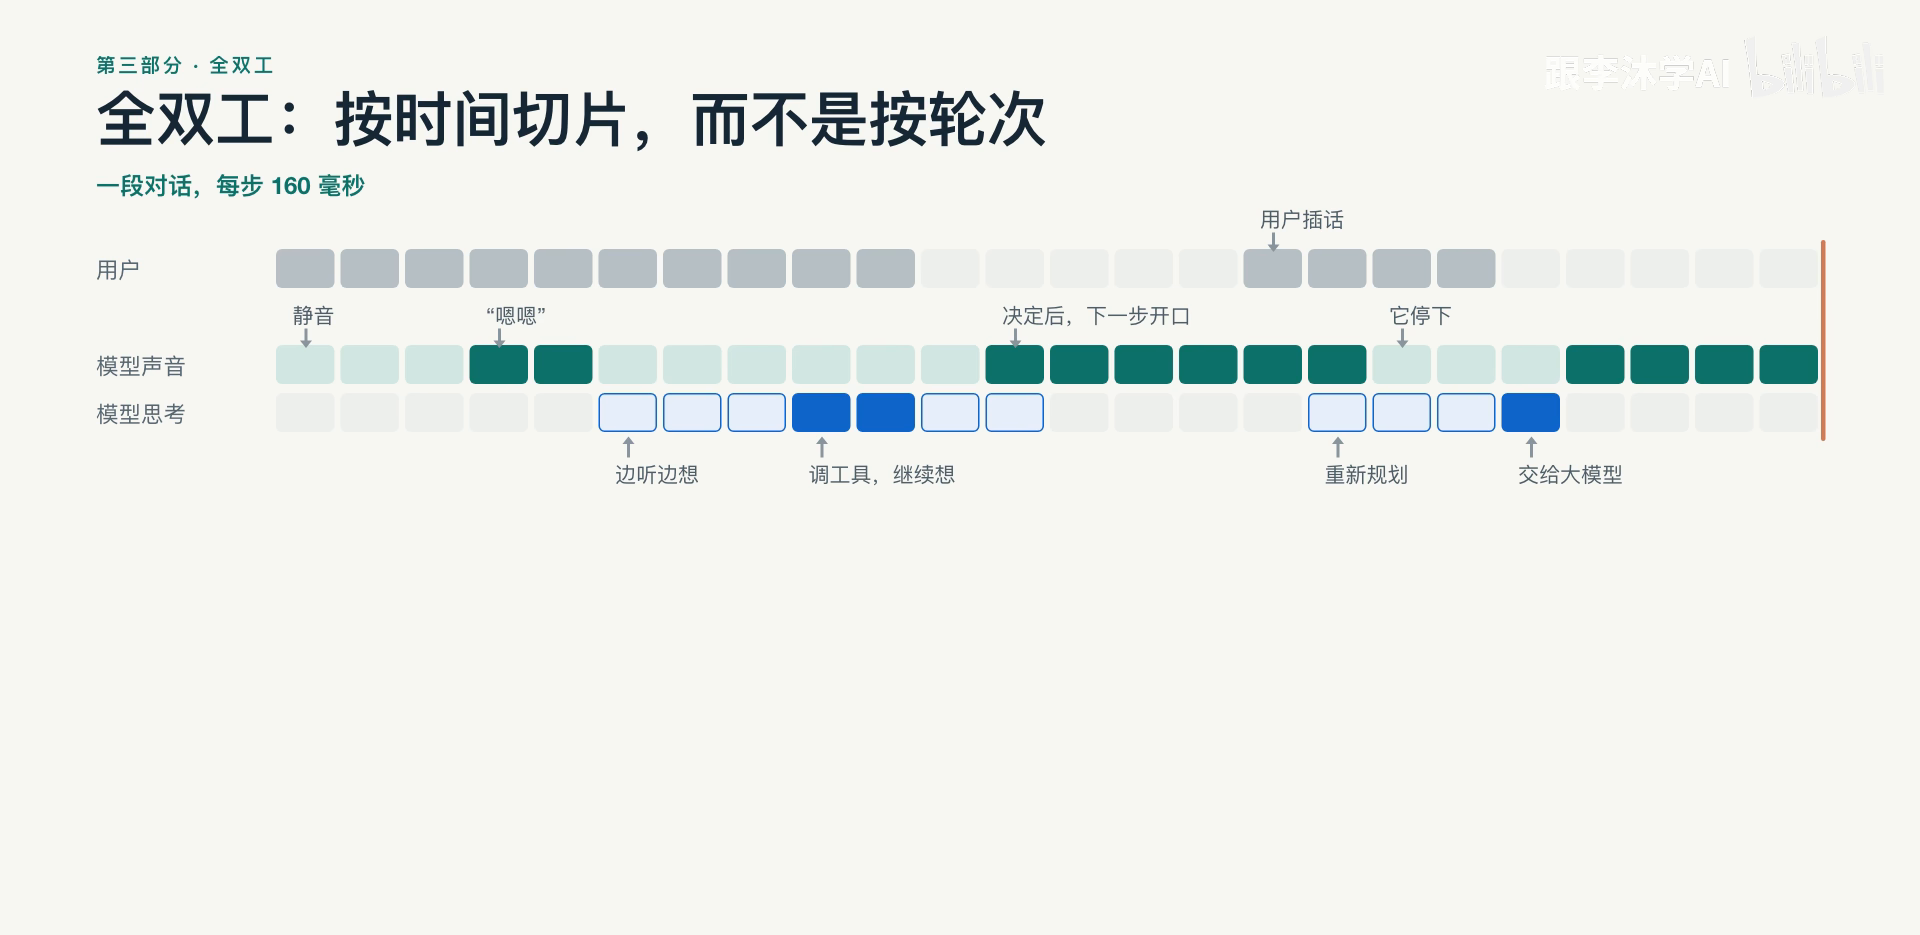
\includegraphics[width=0.95\textwidth]{figures/fig_19_full_duplex_160ms_timeline.png}
\caption{全双工核心时序全景图（每一小格代表 160毫秒）：模型完全抛弃外置 VAD，自主在时间片流中完成倾听静音、中途附和“嗯嗯”、边听边想、后台调工具、开口回答、遇用户插话即停并重新规划委派大模型\vtag}
\end{figure}
\srcnote{00:30:30--00:30:45}

\begin{figure}[H]
\centering
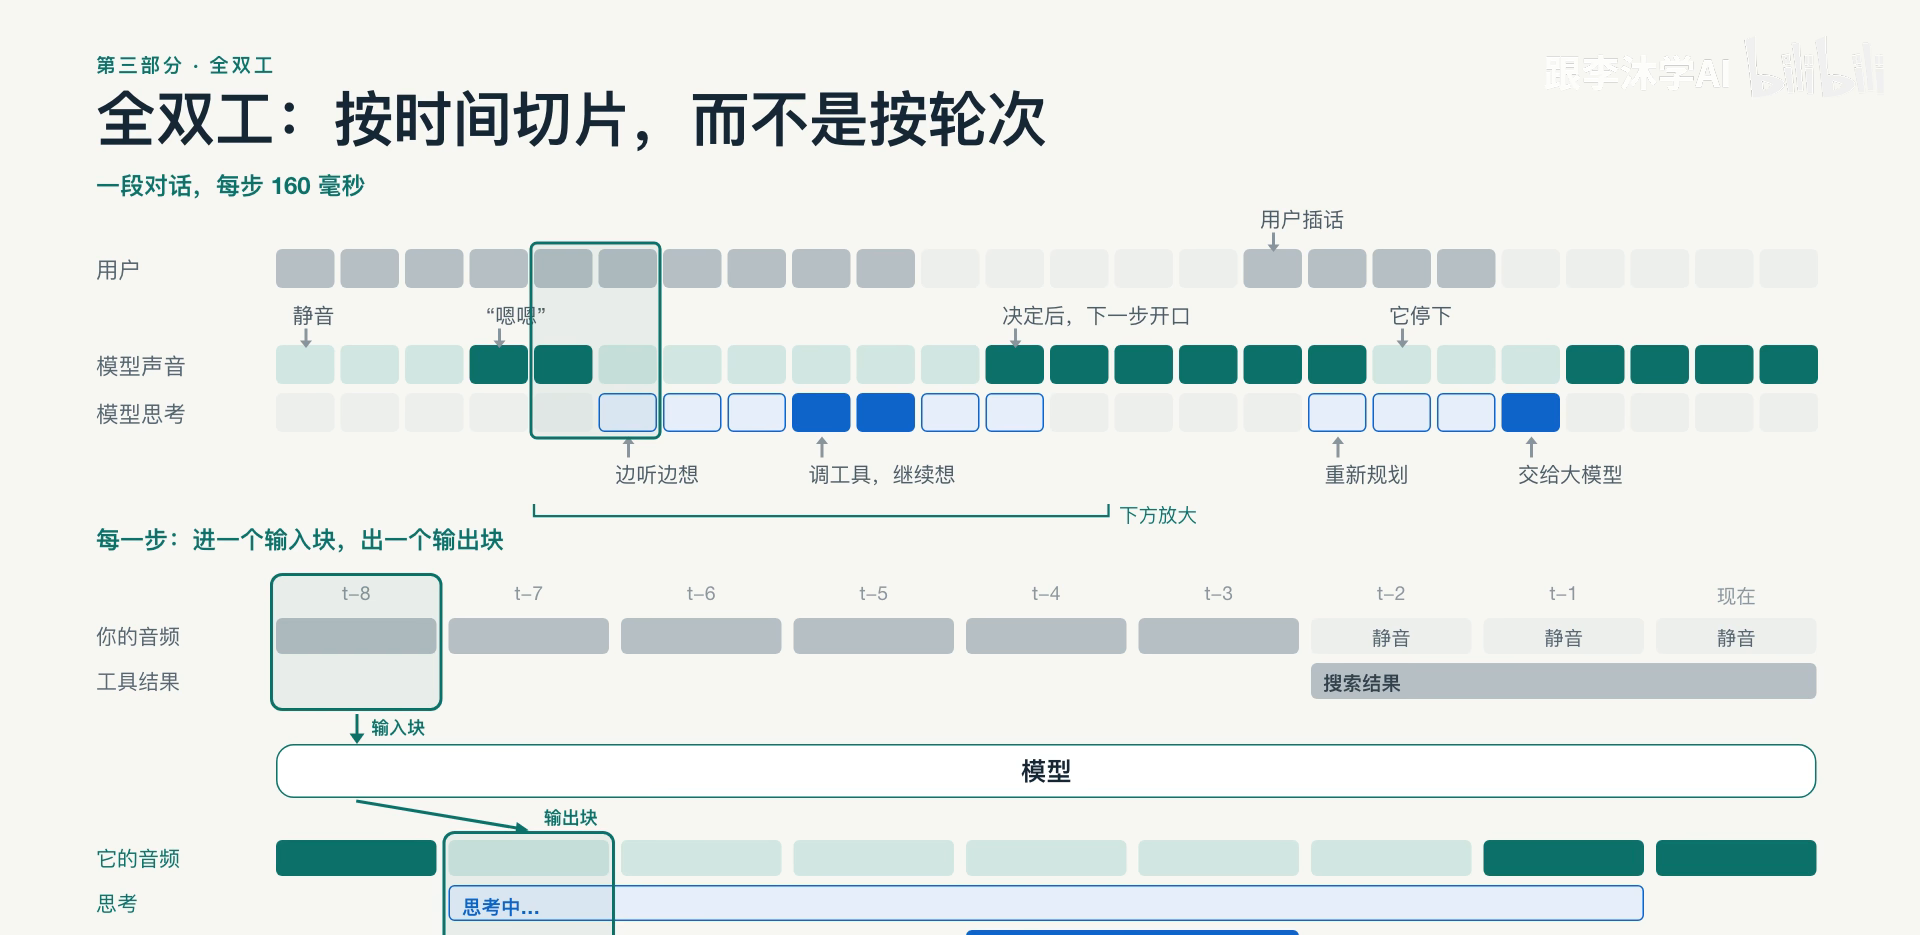
\includegraphics[width=0.95\textwidth]{figures/fig_20_eight_steps_zoom_in.png}
\caption{全双工 8 步时间窗口局部放大（从 $t-8$ 到当前时刻）：每一步进一个输入块、出一个输出块；思考与工具调用跨多个 160毫秒时间片流式拼接，工具返回结果分块注入后续输入流\vtag}
\end{figure}
\srcnote{00:31:45--00:32:00}

沿着图 19 从左到右的时间轴（每一个方格代表 **160毫秒**），我们可以清晰地看到全双工模型是如何把过去死板的轮次交互变成鲜活的多线程交响乐的：
\begin{enumerate}
    \item \textbf{模型自己就是最好的多模态 VAD}：
    在时间轴最左侧，用户正在连续说话（灰色块）。在第 1 到第 3 个时间片，模型判断用户刚起头，因此在“模型声音”轨上输出浅绿色的**静音块**；到了第 4、第 5 个时间片，模型听懂了用户前半句的意思，主动在声音轨输出深绿色的**“嗯嗯（mm-hm）”**附和声，同时在第三行“模型思考”轨上启动了蓝框**边听边想（Thinking）**！
    \item \textbf{用户还没说完，模型已经在后台把工具调完了}：
    当用户继续说后半句时，模型在思考轨上已经猜到了用户需要查询什么信息，提前在蓝色实心块处异步发起了**工具调用（Call Tools）**并继续思考。等到用户话音刚落（灰色块变浅进入静音），外部工具的查询结果刚好返回；模型无需任何等待，在紧接着的下一个 160毫秒时间片立刻决定开口流畅回答（连续深绿色块）！
    \item \textbf{丝滑处理用户中途插话与动态重规划}：
    当模型说到一半时，用户突然开口插话（右侧灰色“用户插话”块）。模型在收到插话音频块的下一个 160毫秒时间片内**当场停止发声**（深绿变浅绿静音），并在思考轨上立即启动**重新规划（Re-plan）**；发现用户的新问题难度较高后，模型一边先开口跟用户自然周旋，一边在后台把难题**委派给后端大模型（Delegate）**！
\end{enumerate}

再看图 20 将其中 8 个连续时间步（$t-8, t-7, \dots, t-1, \text{现在}$）放大后的微观执行细节：
\begin{itemize}
    \item \textbf{跨时间片流式拼接（Chunked Stream Concatenation）}：由于单个时间片只有 160毫秒，模型在单步内只需生成几个思考 Token 或半条函数调用语句（如第 $t-5, t-4$ 步生成 \texttt{search(...)}）；将连续多个输出块中的思考轨与工具轨拼接起来，就自然还原出了完整的长思维链与工具调用指令。
    \item \textbf{分阶段流式接收工具结果（Staged Tool Payload Injection）}：外部工具（如网页搜索或代码执行）往往不是一次性吐出全部结果，而是分阶段返回（如图 20 中工具结果跨越 $t-2, t-1, \text{现在}$ 三个输入块分批流入）。而且工具结果作为输入块的文本载荷注入时，不受音频每块固定 Token 数的限制；**模型甚至不需要等工具把所有结果全部跑完，只要看到第一部分返回结果（Part 1），就可以一边继续思考后续分块，一边先开口向用户播报初步结论！**
\end{itemize}

\begin{knowledgebox}{核心突破总结：160毫秒时间切片如何一举三得？}
\begin{enumerate}
    \item \textbf{彻底干掉外置 VAD}：不再有任何独立的 VAD 模块来硬切音频！到底当前 160毫秒该闭嘴继续听、该附和“嗯哼”、还是该正式回答，全由拥有完整音视频与语义上下文的主模型自己每 160毫秒动态决定；
    \item \textbf{真正实现边听边说与毫秒级打断}：输入流与输出流在每一个 160毫秒时间片上完全对称并行，响应与打断延迟被锁定在单步周期（$0.16\,\mathrm{s}$）量级；
    \item \textbf{思考与工具调用彻底异步化}：后台思考与工具调用成为了与语音输出并行的独立输出轨道，再也不会阻塞前台的实时对话流。
\end{enumerate}
\end{knowledgebox}

\subsection{本章小结}

本章深入剖析了 \texttt{Higgs Realtime Duplex} 的核心全双工架构：通过将连续音视频与文本流切分为 160毫秒（0.16秒）的固定时间片，每一步同步读写多模态输入输出块，从而在单一模型内实现了无外置 VAD 的自主话轮控制、0.1至0.2秒级极速响应，以及跨时间片的流式思考与非阻塞工具调用。

% =========================================================================
% SECTION 5
% =========================================================================
\section{全双工异步大脑：思考（Think）、工具调用（Call Tools）与委派（Delegate）}

\subsection{提升智商的三级火箭：前端自主处理 vs 后端大模型委派}

在全双工时间切片架构下，直接与用户进行 160毫秒级实时音视频交互的模型被称为**前端模型（Front Model）**。那么，怎样让这个前端模型在保持极速响应的同时拥有足够高的“智商”呢？幻灯片第 12 页（图 21）展示了 \texttt{Higgs Realtime Duplex} 提升回答质量的三级机制：**Think（思考）**、**Call tools（调用工具）**与 **Delegate（委派）**。

\begin{figure}[H]
\centering
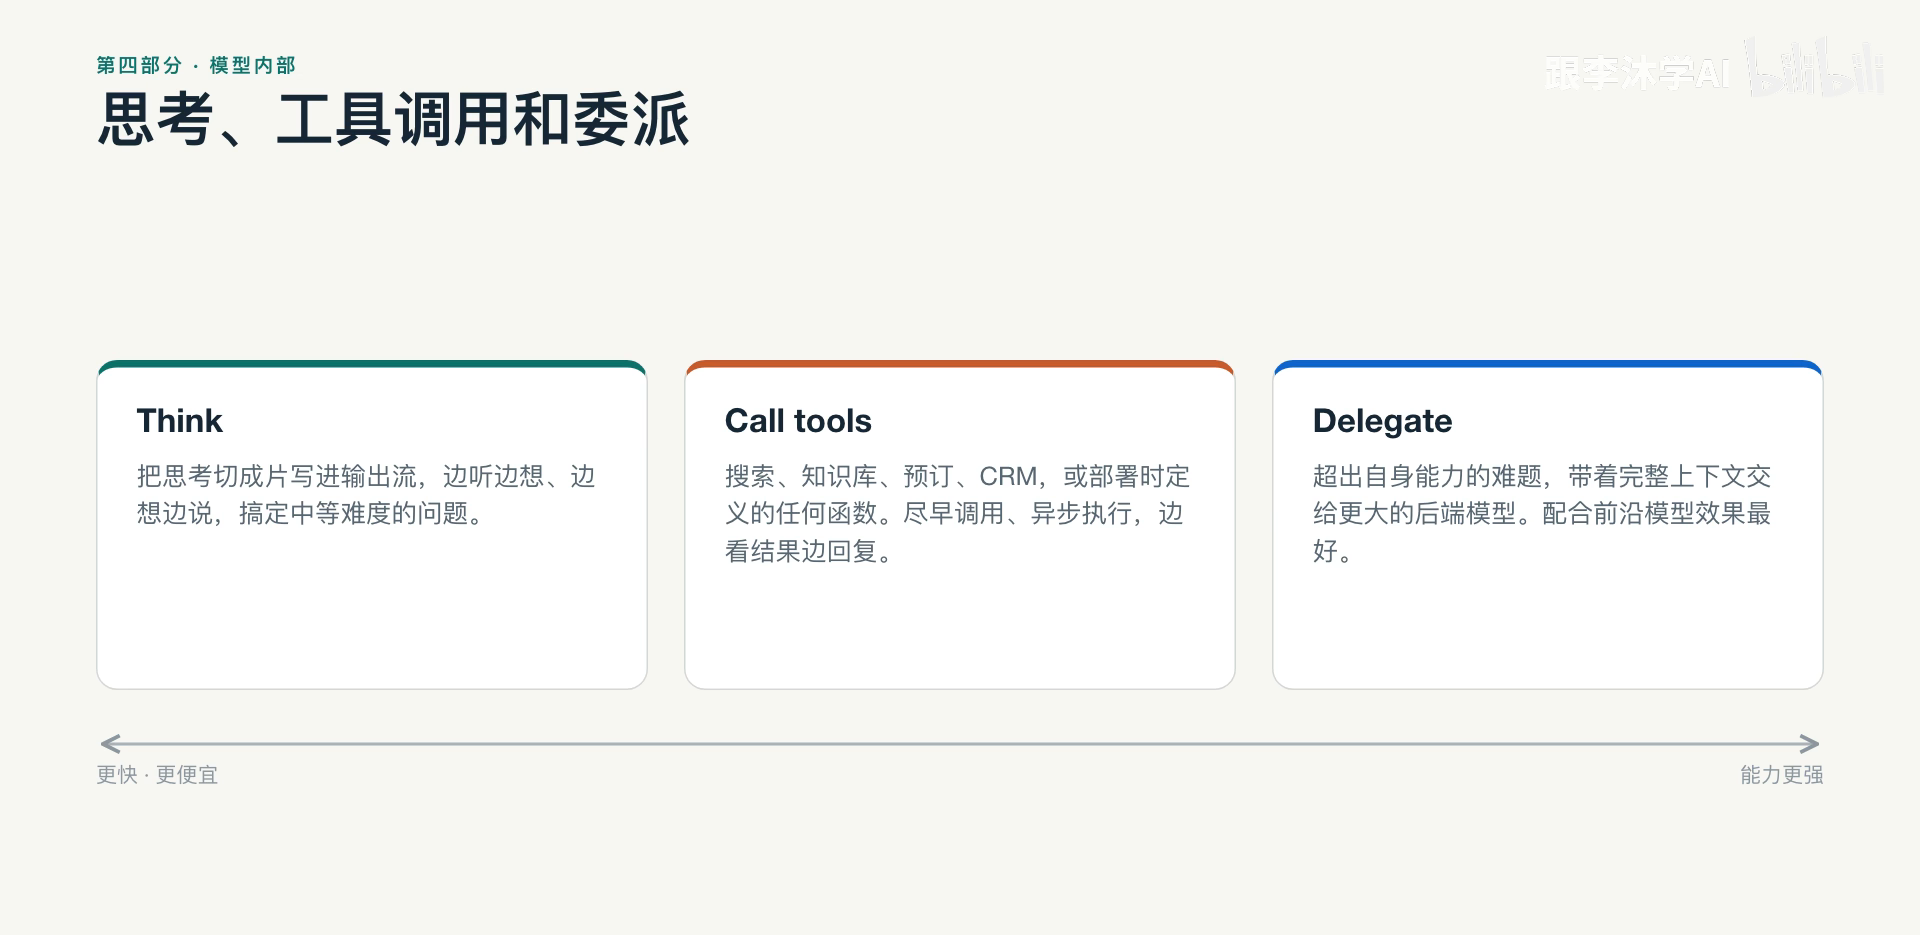
\includegraphics[width=0.95\textwidth]{figures/fig_21_think_call_tools_delegate.png}
\caption{提升模型智商的三种方式：边听边想（Think）、异步调用工具（Call tools）与向更强大后端模型委派（Delegate）\vtag}
\end{figure}
\srcnote{00:33:30--00:33:45}

这三级机制在全双工时间轴上的协同分工如下：
\begin{enumerate}
    \item \textbf{第一级：边听边想（Think）——将数秒钟的推理分摊到用户说话期间}
    深度推理通常需要耗费好几秒钟，但在实时对话里没人愿意每次问完问题都干等好几秒。得益于 160毫秒时间切片，前端模型无需等用户把整段话说完——**每当用户吐出一个有意义的词组或半句话，前端模型就立即在后台思考轨上启动或延续一条推理线程（Reasoning Thread）**。这条思考线程与倾听、说话完全并行，因此模型不仅能“边听边想”，甚至在已经开口回答前半句的同时，脑子里还能继续推演后半句的逻辑！
    \item \textbf{第二级：异步调用工具（Call Tools）——尽早发出请求，基于部分结果先行开口}
    无论是网页搜索、知识库检索、机票预订还是 CRM 客户系统查询，前端模型一旦在倾听中识别出工具需求，就立即以异步方式（Async Call）将工具调用发出去。工具在后台运行期间，前端模型继续正常听看与交谈；一旦工具传回阶段性结果，模型立即将其融入回复，全程零冷场。
    \item \textbf{第三级：向后端大模型委派（Delegate）——好钢用在刀刃上的双模型协同}
    当前端模型遇到超出自身能力边界的超难问题（例如复杂的多步数学证明、大型代码库架构重构或深度长文分析）时，它会将该任务连同完整的共享上下文异步委派给一个**参数量更大、能力更强的后端前沿大模型（Backend Frontier Model）**。在后端大模型埋头苦算的十几秒钟里，前端模型绝不会卡死，而是继续陪用户自然聊天（甚至可以先聊别的话题）；等后端大模型算完传回结果后，前端模型再择机自然地把答案汇报给用户。
\end{enumerate}

\subsection{架构权衡深度对比：为什么不能把所有思考和工具都甩给后端模型？}

在图 21 的讲解中，李沐老师专门对比了几个月前 **Thinking Machines Lab（TML）** 发布的交互模型架构，揭示了一个极其深刻的系统设计权衡：
\begin{itemize}
    \item \textbf{Thinking Machines Lab 的做法（薄前端 $+$ 全量后台委派）}：
    在 TML 的方案中，前端模型只负责最浅层的语音接发与闲聊，把所有的深度思考（Thinking）和工具调用（Tool Calls）统统交给后台大模型去干。这样做的好处是前端模型的训练相对简单；但缺点在实际体验中非常致命：**一个大型推理模型动辄需要思考十来秒钟才能返回结果，如果连查个天气、算个简单账目都要委派给后台大模型，不仅每次交互都要等十来秒才能拿到实质回复，而且每轮都唤醒庞大后端模型会让推理成本高得无法控制！**
    \item \textbf{\texttt{Higgs Realtime Duplex} 的做法（聪明前端自主思考调工具 $+$ 按需低频委派）}：
    Boson AI 坚持让前端模型（45B MoE）自己具备完整的思考（Think）与调用工具（Call Tools）能力，能够独立解决日常 **80\%–90\% 以上** 的常规请求；只有遇到真正棘手的长尾难题（比例 $p_{\mathrm{del}} \ll 1$）时，才动用后端大模型（Delegate）。
\end{itemize}

我们可以用期望延迟 $E[T_{\mathrm{task}}]$ 与期望单轮成本 $E[C_{\mathrm{turn}}]$ 的数学公式直观对比这两种架构：

\begin{equation}
\begin{cases}
E[T_{\mathrm{task}}] = (1 - p_{\mathrm{del}})\,T_{\mathrm{front}} + p_{\mathrm{del}}\,T_{\mathrm{back}}, & T_{\mathrm{front}} \ll T_{\mathrm{back}} \approx 10\,\mathrm{s} \\[6pt]
E[C_{\mathrm{turn}}] = C_{\mathrm{front}} + p_{\mathrm{del}}\,C_{\mathrm{back}}, & p_{\mathrm{del}} \in [0.05, 0.15] \;\ll\; 1
\end{cases}
\end{equation}

上式中，$T_{\mathrm{front}}, C_{\mathrm{front}}$ 分别为前端模型自主思考与调工具的耗时与成本，$T_{\mathrm{back}}, C_{\mathrm{back}}$ 为后端巨型推理模型的耗时与成本，$p_{\mathrm{del}}$ 为触发后端委派的概率。通过让前端模型足够聪明并把 $p_{\mathrm{del}}$ 压到很低，系统在绝大多数轮次中既享受了前端模型的秒级敏捷度，又将单轮平均成本牢牢锁定在轻量级模型的水平！

\begin{importantbox}{架构设计准则：前端模型不能当“传声筒”，必须具备独立 Agent 能力}
在全双工双层架构中，如果前端模型只是一个没有思考与工具调用能力的“传声筒”，它面对用户的实质性问题时就只能反复说“请稍等，我正在帮您查询……”来拖延时间；唯有让前端模型自己能想、自己能调工具，才能在第一时间内给出有信息增量的干货回应。
\end{importantbox}

\subsection{本章小结}

本章拆解了全双工模型提升智商的“思考（Think）—工具调用（Call tools）—后端委派（Delegate）”三级架构，并通过与 Thinking Machines Lab 全量后台委派方案的定量对比，阐明了让前端模型自主承担绝大多数推理与工具调用的延迟与成本优势。

% =========================================================================
% SECTION 6
% =========================================================================
\section{精打细算的 Token 预算与零样本换声换脸（Zero-Shot Voice \& Face）}

\subsection{全双工下的算力危机：如何把每分钟多模态流压到 2.6K Token？}

全双工架构虽然体验极佳，但它带来了一个严峻的工程挑战：**在半双工模型里，只有用户说话时才消耗 Token；而在全双工模型里，哪怕双方都不说话（静音），每 160毫秒也必须照常处理音频输入输出、视频画面输入与数字人面部输出！** 如果不对多模态 Token 速率进行极致压缩，聊上几分钟上下文窗口（Context Window）就会瞬间塞满，推理延迟与显存开销将直接爆炸。

幻灯片第 13 页（图 22）展示了 \texttt{Higgs Realtime Duplex} “精打细算到每一个 Token”的速率设计：

\begin{figure}[H]
\centering
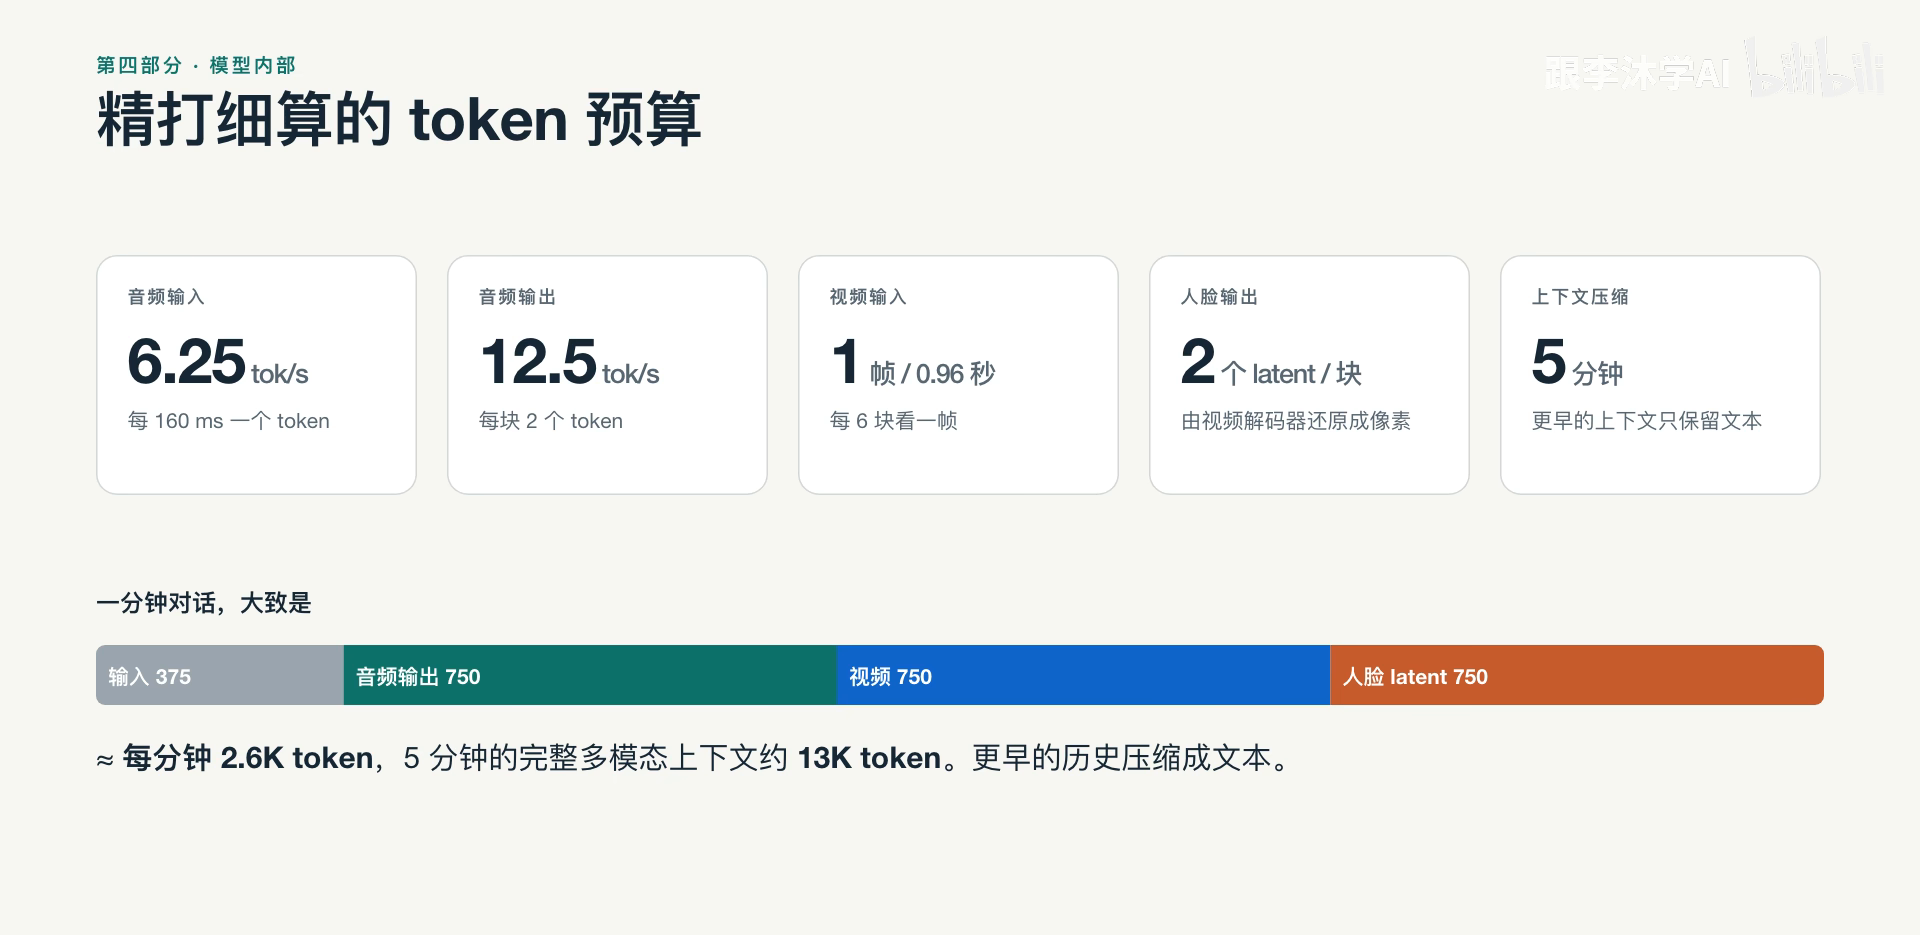
\includegraphics[width=0.95\textwidth]{figures/fig_22_tight_token_budget.png}
\caption{精打细算的 Token 预算：通过极致压缩音频输入（$6.25\,\mathrm{tok/s}$）、音频输出（$12.5\,\mathrm{tok/s}$）、视频抽帧（每 6 块看 1 帧）与人脸输出（每块 2 个 Latent），将每分钟完整音视频流控制在约 $2.6\mathrm{K}$ Token，并配合 5分钟滑动上下文压缩\vtag}
\end{figure}
\srcnote{00:35:15--00:35:30}

让我们严格核算图 22 中的各项多模态流 Token 速率（已知每秒钟包含 $1\,\mathrm{s} / 0.16\,\mathrm{s} = 6.25$ 个时间片，每分钟包含 $60 \times 6.25 = 375$ 个时间片）：
\begin{enumerate}
    \item \textbf{音频输入（Audio In）：$6.25\,\mathrm{tok/s}$（每 160毫秒 仅 $1$ 个 Token）}
    在输入端，音频编码器将每 160毫秒的用户语音高度浓缩为 **$1$ 个音频 Token**。因此每秒钟音频输入仅占 $6.25$ 个 Token，一分钟（375 个时间片）累计僅消耗 $375 \times 1 = \mathbf{375}$ 个 Token！
    \item \textbf{音频输出（Audio Out）：$12.5\,\mathrm{tok/s}$（每 160毫秒 输出 $2$ 个 Token）}
    为什么输出音频比输入音频多一倍？因为输入端只需提取语义与副语言特征供模型理解，而输出端需要还原出高保真、富有韵律细节的声波，因此每 160毫秒时间片分配 **$2$ 个音频 Token**（即每秒 $12.5$ 个 Token），一分钟累计消耗 $375 \times 2 = \mathbf{750}$ 个 Token。
    \item \textbf{视频输入（Video In）：每 6 个时间片（$0.96\text{秒} \approx 1\text{秒}$）采样 $1$ 帧图像}
    在面对面聊天或看共享屏幕时，画面变化没有那么剧烈，根本不需要每秒看 30 帧。系统设定每隔 $6$ 个时间片（即 $6 \times 160\,\mathrm{ms} = 0.96\,\mathrm{s}$，约每秒 1 帧）才读取 $1$ 帧摄像头或屏幕图像，且每帧图像经视觉编码器高度压缩为约 $12$ 个视觉 Token（平均分摊到每个时间片恰好约 $2$ 个 Token），一分钟累计仅消耗约 $\mathbf{750}$ 个 Token！
    \item \textbf{人脸输出（Face Out）：每 160毫秒 输出 $2$ 个视觉隐变量（Latents）}
    为了驱动数字人面部做出同步口型与表情，主模型并不用直接生成庞大的像素矩阵，而是在每个 160毫秒时间片仅输出 **$2$ 个紧凑的面部隐变量（Latents）**，一分钟累计同样仅消耗 $375 \times 2 = \mathbf{750}$ 个 Token。
\end{enumerate}

将以上四项音视频基础流汇总，每分钟的总 Token 消耗速率 $R_{\mathrm{total}}$ 为：

\begin{equation}
R_{\mathrm{total}}
= \underbrace{375}_{\text{音频输入}}
+ \underbrace{750}_{\text{音频输出}}
+ \underbrace{750}_{\text{视频输入}}
+ \underbrace{750}_{\text{人脸}}
+ \underbrace{R_{\mathrm{think/tool}}}_{\text{思考与工具}}
= 2,625 + R_{\mathrm{think/tool}}
\end{equation}

正如课堂幻灯片与口述所指出的：纯音视频流每分钟仅占约 $2,048$ 至 $2,625$（约 $2.6\mathrm{K}$）个 Token，加上动态变化的内部思考、文本与工具调用（每秒几十个 Token），每分钟总消耗也不过 $2.6\mathrm{K}\text{--}5\mathrm{K}$ Token！

更进一步，如果用户跟模型连续聊上几个小时，上下文怎么管理？系统设计了巧妙的**双层滑动窗口与渐进式压缩机制**：
\begin{itemize}
    \item \textbf{最近 5分钟保留完整多模态上下文（约 $13\mathrm{K}\text{--}25\mathrm{K}$ Token）}：对于最近 **5分钟** 内的对话，系统完整保留音频、视频、人脸 Latent 以及经渐进压缩后的思考与工具关键摘要，总长度稳定在 $5 \times 2.6\mathrm{K} \approx 13\mathrm{K}$ 至 $25\mathrm{K}$ Token 之间，让模型对刚刚发生的声学细节与画面记忆犹新；
    \item \textbf{超过 5分钟的早期历史自动退化为纯文本摘要}：一旦某段对话距今超过 5分钟，系统就将其中的原始音频、视频与中间冗长工具轨迹裁掉，仅保留提炼后的纯文本历史记录。这样无论连续聊多少个小时，上下文长度与推理成本都永远不会爆炸！
\end{itemize}

\subsection{零样本换声音与换脸：因果流匹配（Causal Flow Matching）与因果 DiT}

在好交互模型的第一个维度“像人”中，我们希望模型的声音和长相不仅自然，而且可以**由用户或开发者零样本地自由定制（Zero-shot Voice \& Face Cloning）**——给一段几秒钟的参考录音就能换成那个人的声音，给一张单人正面照就能换成那张脸，且完全不需要重新微调（Fine-tune）主模型！幻灯片第 14 页（图 23）展示了实现这一能力的双解码器架构：

\begin{figure}[H]
\centering
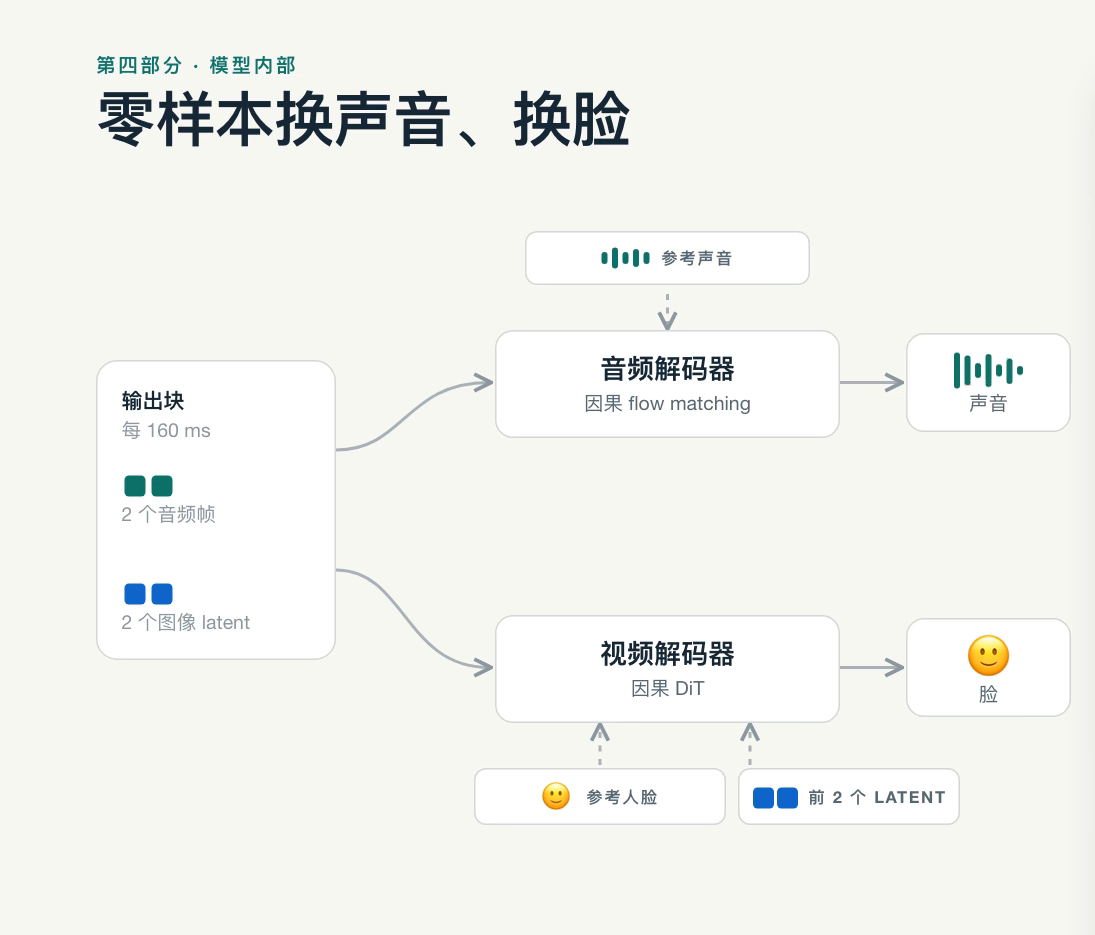
\includegraphics[width=0.76\textwidth]{figures/fig_23_zero_shot_voice_face_decoders.png}
\caption{零样本换声音、换脸架构：主模型每 160毫秒输出与特定音色/面孔解耦的 2 个音频帧与 2 个图像 Latent；末端分别由因果流匹配音频解码器与因果 DiT 视频解码器注入参考音频与参考人脸完成实时渲染\vtag}
\end{figure}
\srcnote{00:36:45--00:37:00}

图 23 的精妙之处在于**“主模型只管内容与神韵，末端解码器负责绑定具体音色与皮相”**：
\begin{enumerate}
    \item \textbf{音色与面孔不烘焙进主模型权重（Decoupled Representation）}：
    45B 前端主模型在每 160毫秒输出的 $2$ 个音频帧（Audio Frames）和 $2$ 个图像隐变量（Image Latents），编码的是“当前这 160毫秒说了什么音素、带什么语气重音、嘴角与眉毛如何运动”，而没有把某一个固定播音员的声纹或长相死死烤进主模型里。
    \item \textbf{音频解码器（Audio Decoder）——因果流匹配（Causal Flow Matching）}：
    在语音端，一个基于**因果流匹配（Causal Flow Matching）**的生成式解码器接收主模型传来的 $2$ 个音频帧，同时将部署时传入的一小段**参考语音（Reference Clip）**编码为条件向量（Conditioning Vector）注入流匹配常微分方程（ODE）积分过程，实时合成与参考音频音色高度一致、同时保留主模型语气神态的语音波形。
    \item \textbf{视频解码器（Video Decoder）——带历史隐变量条件化的因果 DiT（Causal Diffusion Transformer）}：
    由于人脸视频需要极高的空间纹理细节与跨帧时间连续性，视频端采用了一个基于**因果扩散 Transformer（Causal DiT）**的解码器。在每个 160毫秒时间步 $t$，视频解码器不仅以单张**参考人脸图像（Reference Image）** $I_{\mathrm{ref}}$ 和当前主模型输出的 $2$ 个面部隐变量 $z_t^{(1)}, z_t^{(2)}$ 为条件，还显式引入了**前一个时间片的 2 个历史隐变量 $z_{t-1}^{(1)}, z_{t-1}^{(2)}$** 作为自回归时间锚点：
\end{enumerate}

\begin{equation}
\begin{cases}
\hat{w}_t^{\mathrm{speech}} = \mathcal{D}_{\mathrm{audio}}^{\mathrm{CFM}}\Big(a_t^{(1)}, a_t^{(2)}\;\Big|\;\mathrm{Enc}_{\mathrm{spk}}(w_{\mathrm{ref}})\Big) \\[8pt]
\hat{V}_t^{\mathrm{face}} = \mathcal{D}_{\mathrm{video}}^{\mathrm{DiT}}\Big(z_t^{(1)}, z_t^{(2)}\;\Big|\;I_{\mathrm{ref}},\; z_{t-1}^{(1)}, z_{t-1}^{(2)}\Big)
\end{cases}
\end{equation}

上式中，$\mathcal{D}_{\mathrm{audio}}^{\mathrm{CFM}}$ 为因果流匹配音频解码器，$\mathcal{D}_{\mathrm{video}}^{\mathrm{DiT}}$ 为因果 DiT 视频解码器。通过将前两帧隐变量 $(z_{t-1}^{(1)}, z_{t-1}^{(2)})$ 纳入条件输入，生成的数字人面部视频在长达数十分钟的对话中始终保持头部姿态平滑过渡与五官身份高度一致，绝不会在时间片交界处发生画面闪烁或人脸变形！而在切换角色时，只需替换 $(w_{\mathrm{ref}}, I_{\mathrm{ref}})$，即可零成本实现零样本换声换脸。

\subsection{本章小结}

本章算清了全双工架构的经济账：通过将音频输入压至 $6.25\,\mathrm{tok/s}$、音频输出压至 $12.5\,\mathrm{tok/s}$、视频每 6 块抽 1 帧、人脸每块 2 个 Latent，将每分钟音视频流控制在约 $2.6\mathrm{K}$ Token，并配合 5分钟滑动多模态窗口（约 $13\mathrm{K}$ Token）避免长对话爆炸；同时详解了基于因果流匹配与因果 DiT 的零样本换声换脸双解码器机制。

% =========================================================================
% SECTION 7
% =========================================================================
\section{模型与训练：45B MoE、2T 中期训练、GRPO 多教师蒸馏与 RSI 闭环}

\subsection{为什么选择 45B MoE？以及 2 万亿 Token 多模态中期训练（Mid-Training）}

进入讲座第四部分“模型内部”（图 24、图 25），李沐老师揭秘了 \texttt{Higgs Realtime Duplex} 的模型规模选型与三阶段训练流水线。

\begin{figure}[H]
\centering
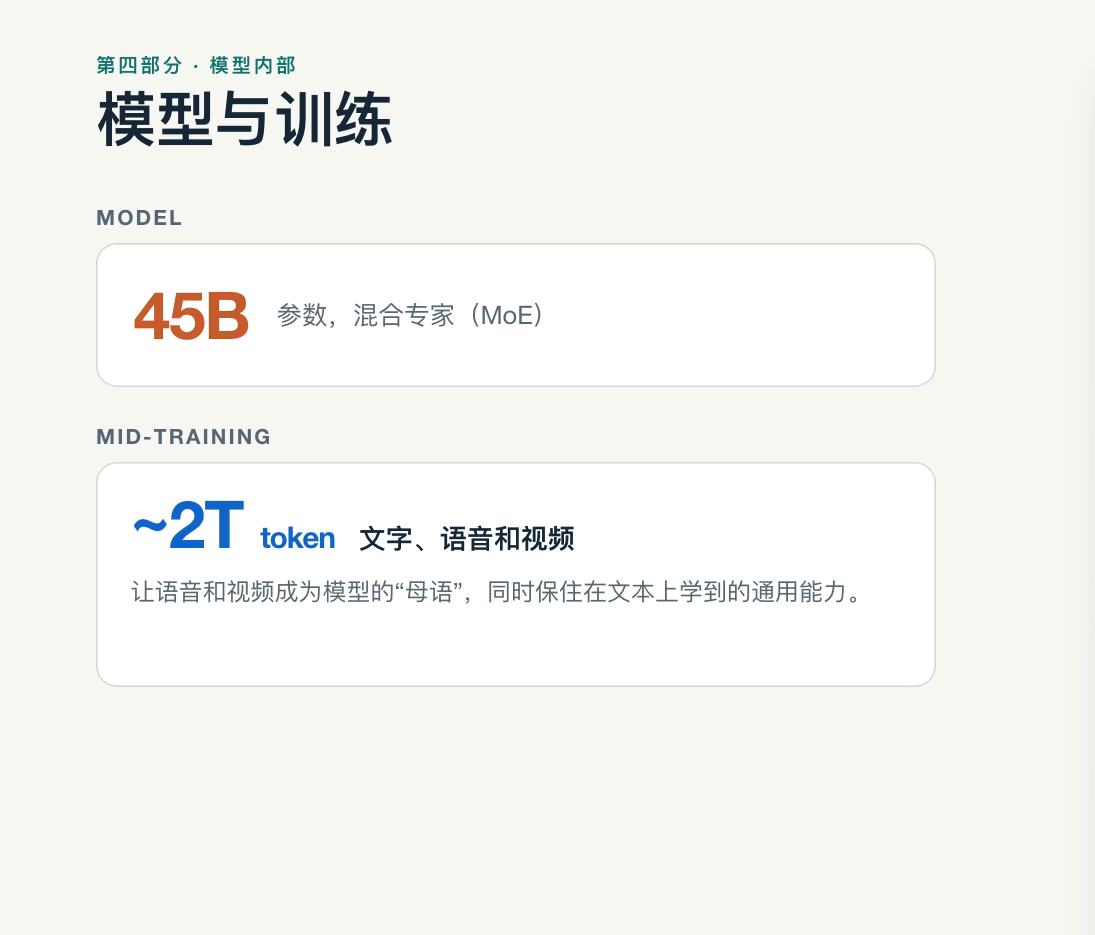
\includegraphics[width=0.74\textwidth]{figures/fig_24_model_45b_moe_2t_midtrain.png}
\caption{模型与训练（一）：采用 45B 参数混合专家（MoE）模型作为主模型，并在约 2T（2 万亿）Token 的文本、语音和视频混合语料上进行中期训练（Mid-training）\vtag}
\end{figure}
\srcnote{00:38:30--00:38:45}

\begin{figure}[H]
\centering
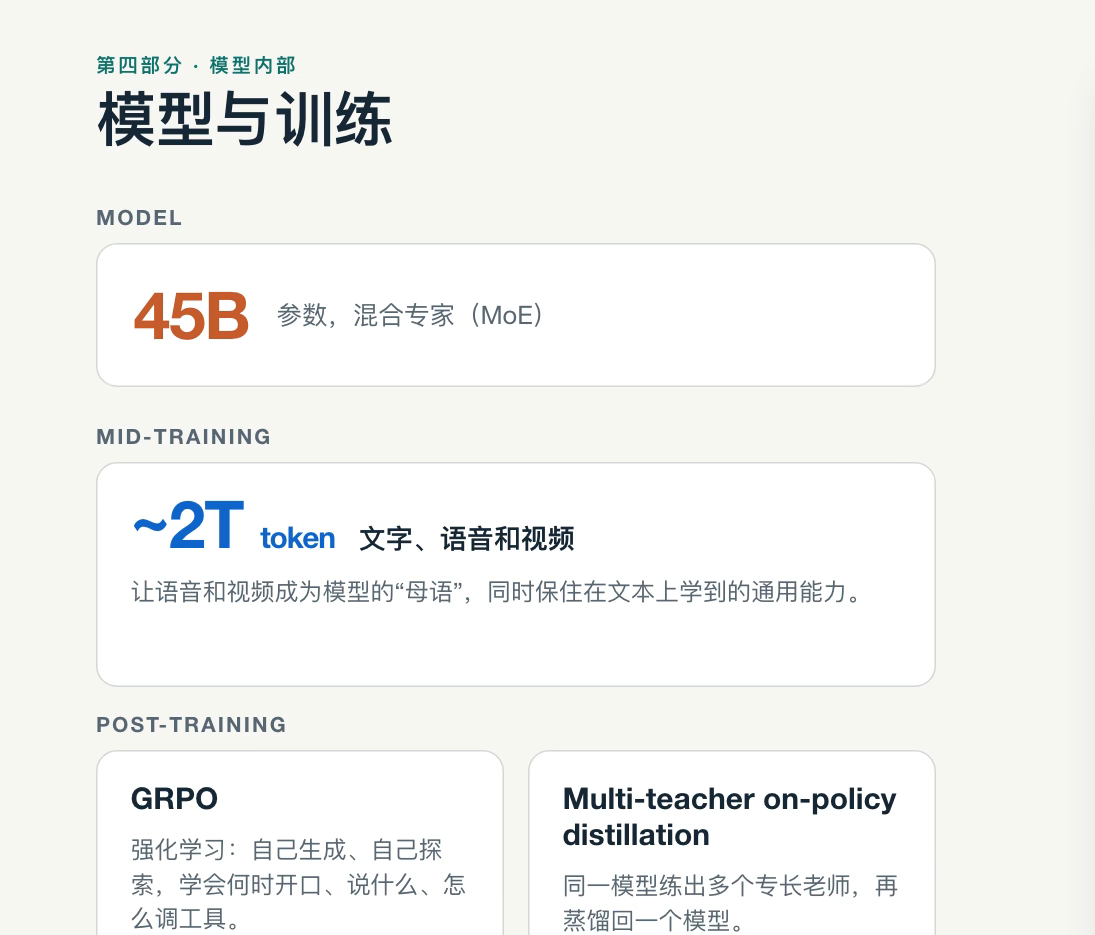
\includegraphics[width=0.74\textwidth]{figures/fig_25_posttrain_grpo_mopd_rsi.png}
\caption{模型与训练（二）：后训练（Post-training）结合 GRPO 强化学习与多教师在线蒸馏（Multi-teacher On-Policy Distillation），将多个专项教师的能力汇聚到单一学生模型中\vtag}
\end{figure}
\srcnote{00:39:30--00:39:45}

\subsubsection{模型选型：45B 混合专家模型（Mixture-of-Experts，MoE）的黄金平衡点}
前端模型到底应该做多大？如果用几十亿参数（如 7B/8B）的稠密小模型，虽然跑得快，但情商与智商明显不够用，稍微复杂一点的指令就听不懂；反过来，Boson AI 团队也尝试过训练更大尺寸的模型——大模型的评测分数确实更高，但每 160毫秒都要前向推理一次的算力成本太高了。考虑到真正极其困难的长尾问题本来就可以通过 `Delegate` 异步交给后端巨型模型处理，团队最终选择了 **45B 总参数的混合专家模型（45B MoE）** 作为前端主模型：利用 MoE 稀疏激活的特性，它兼具中等偏上规模模型的扎实智商与小激活参数模型的极速推理吞吐，完美契合 160毫秒时间片的实时预算。

\subsubsection{中期训练（Mid-Training）：约 2T（2 万亿）Token 打通三模态语义空间}
团队从一个经过充分文本预训练的 45B MoE 基座模型出发，在 Boson AI 自建数据中心的 NVIDIA H100 集群上（基于定制化的 Megatron 分布式训练栈），投入了约 **2T（2 万亿）Token 的文本、语音和视频混合数据**进行中期训练（Mid-training）：
\begin{itemize}
    \item \textbf{为什么中期训练还要保留大量纯文本 Token？} 因为模型的高阶逻辑推理与世界知识主要是在纯文本上习得的；如果在中期训练中只喂音视频数据，模型就会发生灾难性遗忘（Catastrophic Forgetting），变成“四肢发达、头脑简单”的语音复读机。持续混入高比例文本能牢牢保住基座的通用智商。
    \item \textbf{打通语音、视频与文字的原生跨模态对齐}：海量的交织音视频与文本数据让模型学会直接理解原始声学与视觉表征，把“听到的声音”、“看到的画面”与“说出的话语”在同一个隐空间中彻底对齐。
\end{itemize}

\subsection{后训练秘籍：GRPO 强化学习、多教师在线蒸馏（MOPD）与 RSI 仿真闭环}

经过 2T Token 中期训练后，模型虽然懂了多模态知识，但要让它在 160毫秒全双工流中学会**“什么时候该插话、什么时候该闭嘴、什么时候该边听边想、什么时候该调工具或委派大模型”**，最关键的决胜场在于**后训练（Post-training）**（图 25）！

为什么全双工后训练极其困难？因为全双工模型要同时兼顾太多互相冲突的任务目标：既要自然闲聊附和，又要精准遵守指令，还要做异步工具调用与动态委派。如果直接用一套混合奖励函数在一个模型上硬跑强化学习（RL），不同任务梯度很容易互相打架（跷跷板效应），而且为每一种子任务单独搭建复杂的实时交互仿真环境成本极高。

为此，Boson AI 采用了两项核心后训练技术：

\subsubsection{技术一：GRPO $+$ 多教师在线蒸馏（Multi-Teacher On-Policy Distillation，MOPD）}
团队没有试图用单次 RL 一步登天，而是采用了**“分科培养专精名师 $\to$ 在线同源蒸馏全能学生”**的策略：
\begin{enumerate}
    \item \textbf{用 GRPO 训练多个专精教师模型（Specialist Teachers）}：
    从**同一个 45B MoE 基础模型**出发，针对不同任务簇（自然对话节奏、全双工打断与附和交互、动态工具调用与后端委派、复杂任务完成度）分别构建强化学习环境，使用 **GRPO（Group Relative Policy Optimization）** 算法训练出多个在各自领域拿到极高分数的专精教师策略 $\{\pi_{\mathrm{teacher}}^{(k)}\}_{k=1}^K$。
    \item \textbf{多教师在线策略蒸馏（MOPD）合流为单一学生模型}：
    随后，训练最终部署的单一学生模型 $\pi_{\theta}$。所谓**在线蒸馏（On-Policy Distillation）**，是指在训练时由**学生模型自己**在交互环境中采样生成轨迹 $\tau \sim \pi_{\theta}$，但在每个时间步上，由对应领域的专精教师模型 $\pi_{\mathrm{teacher}}^{(k)}$ 对学生当前状态的动作分布提供 Token 级分布指导（最小化学生与专精教师之间的逆向或前向 KL 散度）：
\end{enumerate}

\begin{equation}
\mathcal{L}_{\mathrm{MOPD}}(\theta)
= \sum_{k=1}^K w_k\,\mathbb{E}_{\tau \sim \pi_{\theta}^{(k)}}\!\left[
\sum_{t=1}^{|\tau|} D_{\mathrm{KL}}\!\Big(\pi_{\mathrm{teacher}}^{(k)}(\cdot \mid s_t)\;\Big\|\;\pi_{\theta}(\cdot \mid s_t)\Big)
\right]
\end{equation}

李沐老师在视频中特别点出了一个至关重要的工程经验：**在做多教师蒸馏时，所有的专精教师模型最好是从同一个基座模型（Same Base Model Family）长出来的！** 因为同源家族模型内部的表征空间与 Token 概率分布具有天然的相似性，当多个同源教师一起去教同一个学生模型时，概率分布不会发生剧烈的结构冲突，学生的蒸馏收敛会顺滑、容易得多！

\subsubsection{技术二：递归自我改进（Recursive Self-Improvement，RSI）交互仿真闭环}
除了 MOPD，官方技术报告还披露了支撑这套系统持续进化的**递归自我改进（RSI）闭环**：
\begin{itemize}
    \item \textbf{工程核心是构建全套仿真器（Simulator Harness）而非孤立调模型}：团队构建了一套高拟真的全双工交互仿真环境，能够逼真复现真实人类对话中的各种极端路况——中途突然打断（Interruptions）、双人抢话重叠音（Overlapping Speech）、跟旁人说话的侧边交谈（Side Conversations）以及复杂背景噪音。
    \item \textbf{自动化“交互 $\to$ 审视失败 $\to$ 合成针对性数据 $\to$ 重训练”循环}：Agent 在仿真环境中大规模自博弈交互，由自动裁判（Judges）挑出模型抢话、漏听或工具调用失败的坏例（Edge Cases），自动合成针对性修正训练数据并迭代更新模型，使精干的研发团队无需海量人工标注即可快速攻克长尾交互缺陷。
\end{itemize}

\begin{knowledgebox}{后训练核心方法论：为什么全双工模型必须靠 RL + 仿真环境训练？}
传统的静态语音问答数据集只有“一问一答”的干净录音，里面根本没有“用户说到一半喘气 $0.34\,\mathrm{s}$”、“用户转头跟店员点汉堡”或“工具分三批返回结果时边想边说”的动态时序轨迹。只有把模型放进可交互的实时仿真环境里跑 GRPO 强化学习，再用 MOPD 把各路专精教师汇于一身，模型才能真正长出全双工的“时间感”与“分寸感”。
\end{knowledgebox}

\subsection{本章小结}

本章深入解析了 \texttt{Higgs Realtime Duplex} 的模型与训练体系：选用 45B MoE 平衡前端算力与智商，经 2T Token 多模态中期训练打通文本、语音与视觉表征，再通过同源家族 GRPO 专精教师的多教师在线蒸馏（MOPD）与递归自我改进（RSI）仿真闭环赋予模型全双工交互能力。

% =========================================================================
% SECTION 8
% =========================================================================
\section{权威基准评测与全讲总结：小而精的 45B MoE 何以匹敌 6 倍巨头？}

\subsection{七大权威基准全面交锋：45B MoE 对战 276B TML、GPT 与 Gemini}

训出来的 \texttt{Higgs Realtime Duplex}（45B MoE）实际水平究竟如何？幻灯片第 16 页（图 26）与官方技术报告给出了它与几个月前发布的 **Thinking Machines Lab（TML）Interaction Small（276B MoE）**、**OpenAI GPT Realtime \& Live 系列**以及 **Google Gemini Live 系列**在七大权威多模态与语音基准上的全面对比（表 1）：

\begin{figure}[H]
\centering
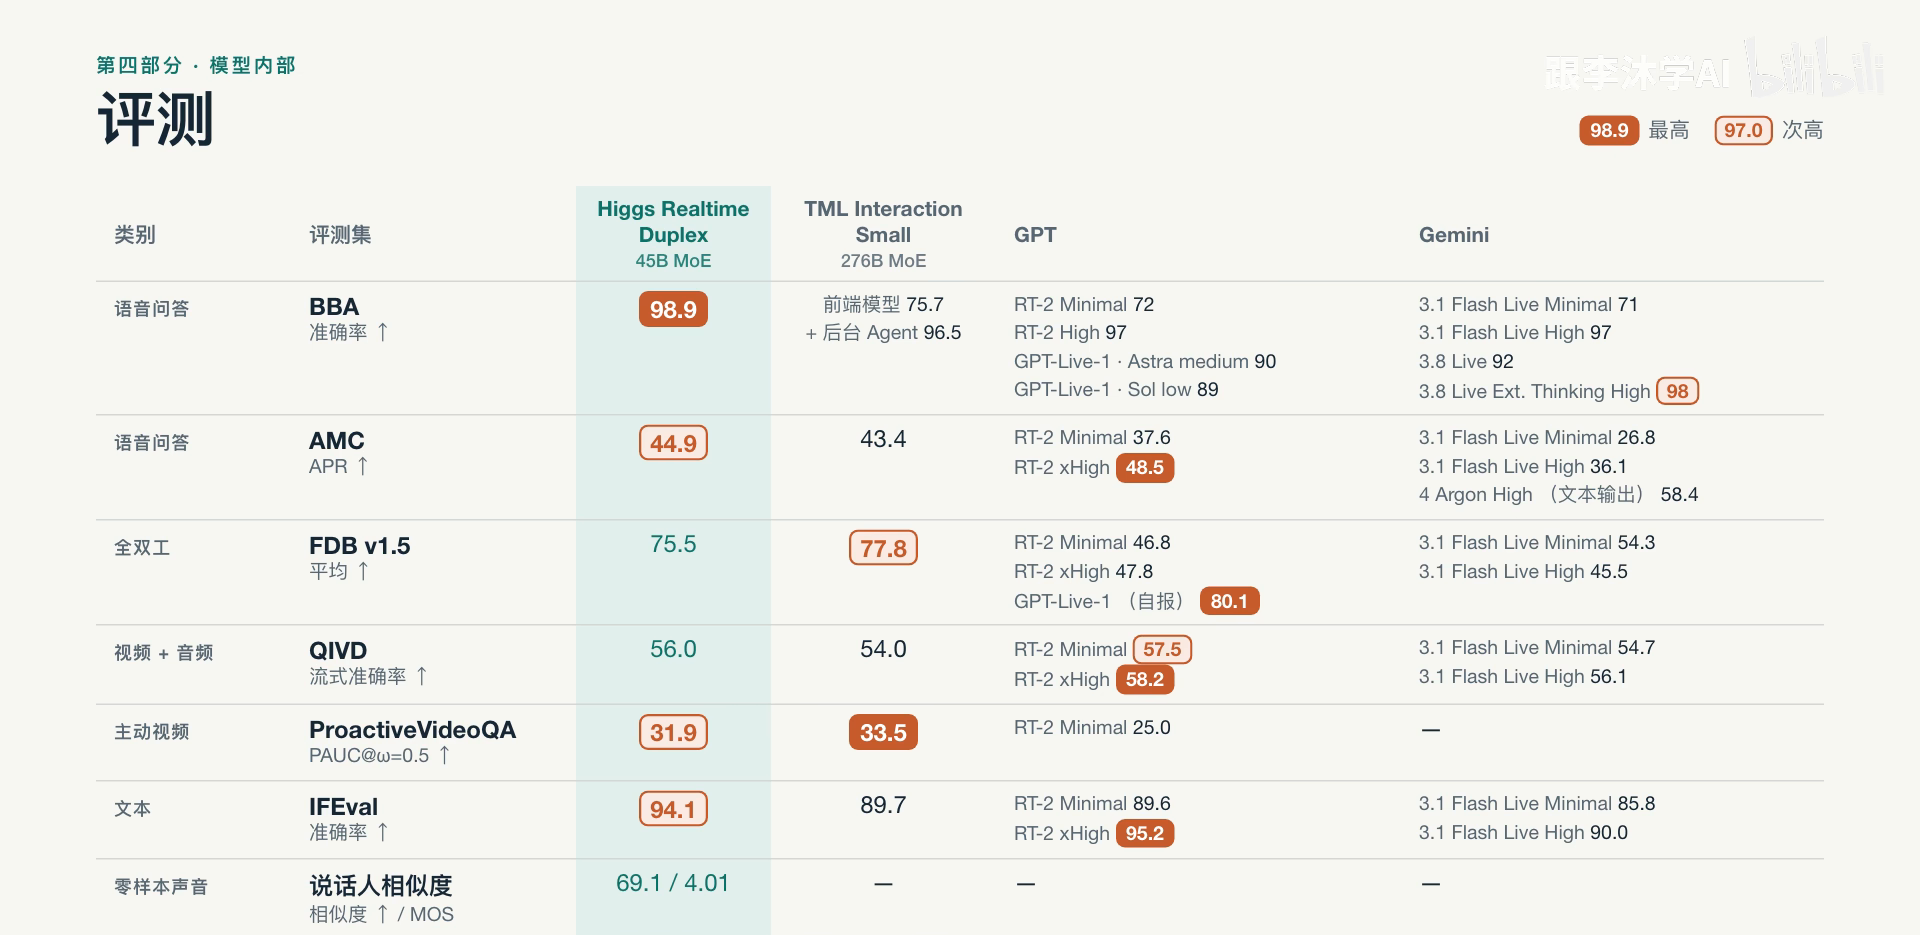
\includegraphics[width=0.95\textwidth]{figures/fig_26_benchmark_comparison_table.png}
\caption{综合评测对比表：Higgs Realtime Duplex（45B MoE）与 TML Interaction Small（276B MoE）、GPT Realtime/Live 系列及 Gemini Live 系列在语音问答、全双工交互、音视频理解、主动视频、文本指令遵循与零样本声音克隆上的全面对比（实心红框为全场最高分，空心红框为全场次高分）\vtag}
\end{figure}
\srcnote{00:40:45--00:41:00}

\begin{table}[H]
\centering
\small
\caption{Higgs Realtime Duplex 与主流实时/全双工模型在核心基准上的评测结果对照表}
\begin{tabular}{p{2.0cm}p{2.4cm}p{1.8cm}p{2.1cm}p{2.4cm}p{2.3cm}}
\toprule
\textbf{评测类别} & \textbf{基准集与指标} & \textbf{Higgs Duplex (45B MoE)} & \textbf{TML Small (276B MoE)} & \textbf{OpenAI GPT Realtime / Live} & \textbf{Google Gemini Live 系列} \\
\midrule
\textbf{语音问答} & \textbf{Big Bench Audio (BBA)} 准确率 $\uparrow$ & \textbf{98.9}（全场最高） & 96.5（前端 75.7 $+$ 后台 96.5） & RT-2 Min: 72 / High: 97; Live-1: 90 & 3.1 Min: 71 / High: 97; 3.8 Ext: \textbf{98} \\
\textbf{语音多轮挑战} & \textbf{Audio Multi\-Challenge (AMC)} APR $\uparrow$ & \textbf{44.9}（全场次高） & 43.4 & RT-2 Min: 37.6 / xHigh: \textbf{48.5} & 3.1 Min: 26.8 / High: 36.1 \\
\textbf{全双工综合} & \textbf{Full-Duplex-Bench v1.5} 平均分 $\uparrow$ & \textbf{75.5} & \textbf{77.8}（次高） & RT-2 Min: 46.8 / xHigh: 47.8; Live-1: \textbf{80.1} & 3.1 Min: 54.3 / High: 45.5 \\
\textbf{视频$+$音频理解} & \textbf{QIVD} 流式准确率 $\uparrow$ & \textbf{56.0} & 54.0 & RT-2 Min: \textbf{57.5} / xHigh: \textbf{58.2} & 3.1 Min: 54.7 / High: 56.1 \\
\textbf{主动视频交互} & \textbf{Proactive\-VideoQA} PAUC $\uparrow$ & \textbf{31.9}（全场次高） & \textbf{33.5}（最高） & RT-2 Min: 25.0 & —（未运行/不支持） \\
\textbf{语音工具 Agent} & \textbf{$\tau$-Voice} 任务完成率 pass@1 (\%) $\uparrow$ & \textbf{69.8}（全场次高） & —（未运行） & RT-2 Min: 30.8 / High: 39.8; Live-1: \textbf{74.5} & 3.1 Min: 26.2 / High: 37.7; 3.8 Ext: 68.6 \\
\textbf{文本指令遵循} & \textbf{IFEval} 准确率 $\uparrow$ & \textbf{94.1}（全场次高） & 89.7 & RT-2 Min: 89.6 / xHigh: \textbf{95.2} & 3.1 Min: 85.8 / High: 90.0 \\
\textbf{零样本声音克隆} & \textbf{说话人相似度} Sim $\uparrow$ / MOS $\uparrow$ & \textbf{69.1 / 4.01} & —（不支持） & —（不支持） & —（不支持） \\
\bottomrule
\end{tabular}
\end{table}

结合图 26 与表 1 的数据，李沐老师提炼出了两个极具启发性的核心观察：
\begin{enumerate}
    \item \textbf{高思考档位（Thinking High）对语音评测至关重要，且前端独立能力差距悬殊}：
    仔细看 GPT（如 `RT-2 Minimal` vs `RT-2 High/xHigh`）和 Gemini（`3.1 Flash Live Minimal` vs `High`）的分数可以发现：一旦把 Thinking 关小（Minimal），它们在 Big Bench Audio 上的准确率立刻暴跌到 $71\text{--}72$ 分，在 $\tau$-Voice 工具调用上更是跌到 $26.2\%\text{--}30.8\%$；只有把 Thinking 开到最高档，分数才能拉回 $97\text{--}98$ 分。同样地，看 TML Interaction Small 在 BBA 上的表现：如果不调后台 Agent、只靠前端模型自己答，准确率只有 $75.7\%$，必须加上后台 Agent 才能到 $96.5\%$；而 \textbf{\texttt{Higgs Realtime Duplex} 直接在全双工流式状态下拿到了全场最高分 $98.9\%$}，并在 AMC、ProactiveVideoQA、$\tau$-Voice 和 IFEval 上悉数斩获全场次高分！
    \item \textbf{45B MoE 越级挑战大将近 6倍的 276B MoE——全双工领域仍处于“架构与数据为王”的早期阶段}：
    最令人振奋的对比在于模型体积：\texttt{Higgs Realtime Duplex} 的前端模型只有 **45B 参数**，而 Thinking Machines Lab 的 `Interaction Small` 高达 **276B 参数——参数量大了将近 6倍**（OpenAI 与 Google 的旗舰模型体积据信也远大于 45B）！然而在全部七项基准上，45B 的 \texttt{Higgs Realtime Duplex} 与 276B 的 TML 杀得有来有回、甚至在多项指标上反超，同时还独家支持零样本声音克隆（说话人相似度 $69.1$，MOS 自然度评分 $4.01$）与零样本数字人换脸！
    这有力地证明了：**全双工多模态交互目前依然处于技术演进的早期阶段；在这个阶段，精巧的 160毫秒时间切片架构、高质量合成交互数据以及 GRPO+MOPD 后训练方法，比单纯靠暴力堆叠模型参数量（Raw Scale）重要得多！**
\end{enumerate}

\subsection{回到黄金三角：全讲技术全景总结与展望}

在讲座最后（图 27、图 28），李沐老师将整套技术方案重新映射回开篇提出的“像人、够聪明、成本低”黄金三角，形成了一张严丝合缝的工程答卷：

\begin{figure}[H]
\centering
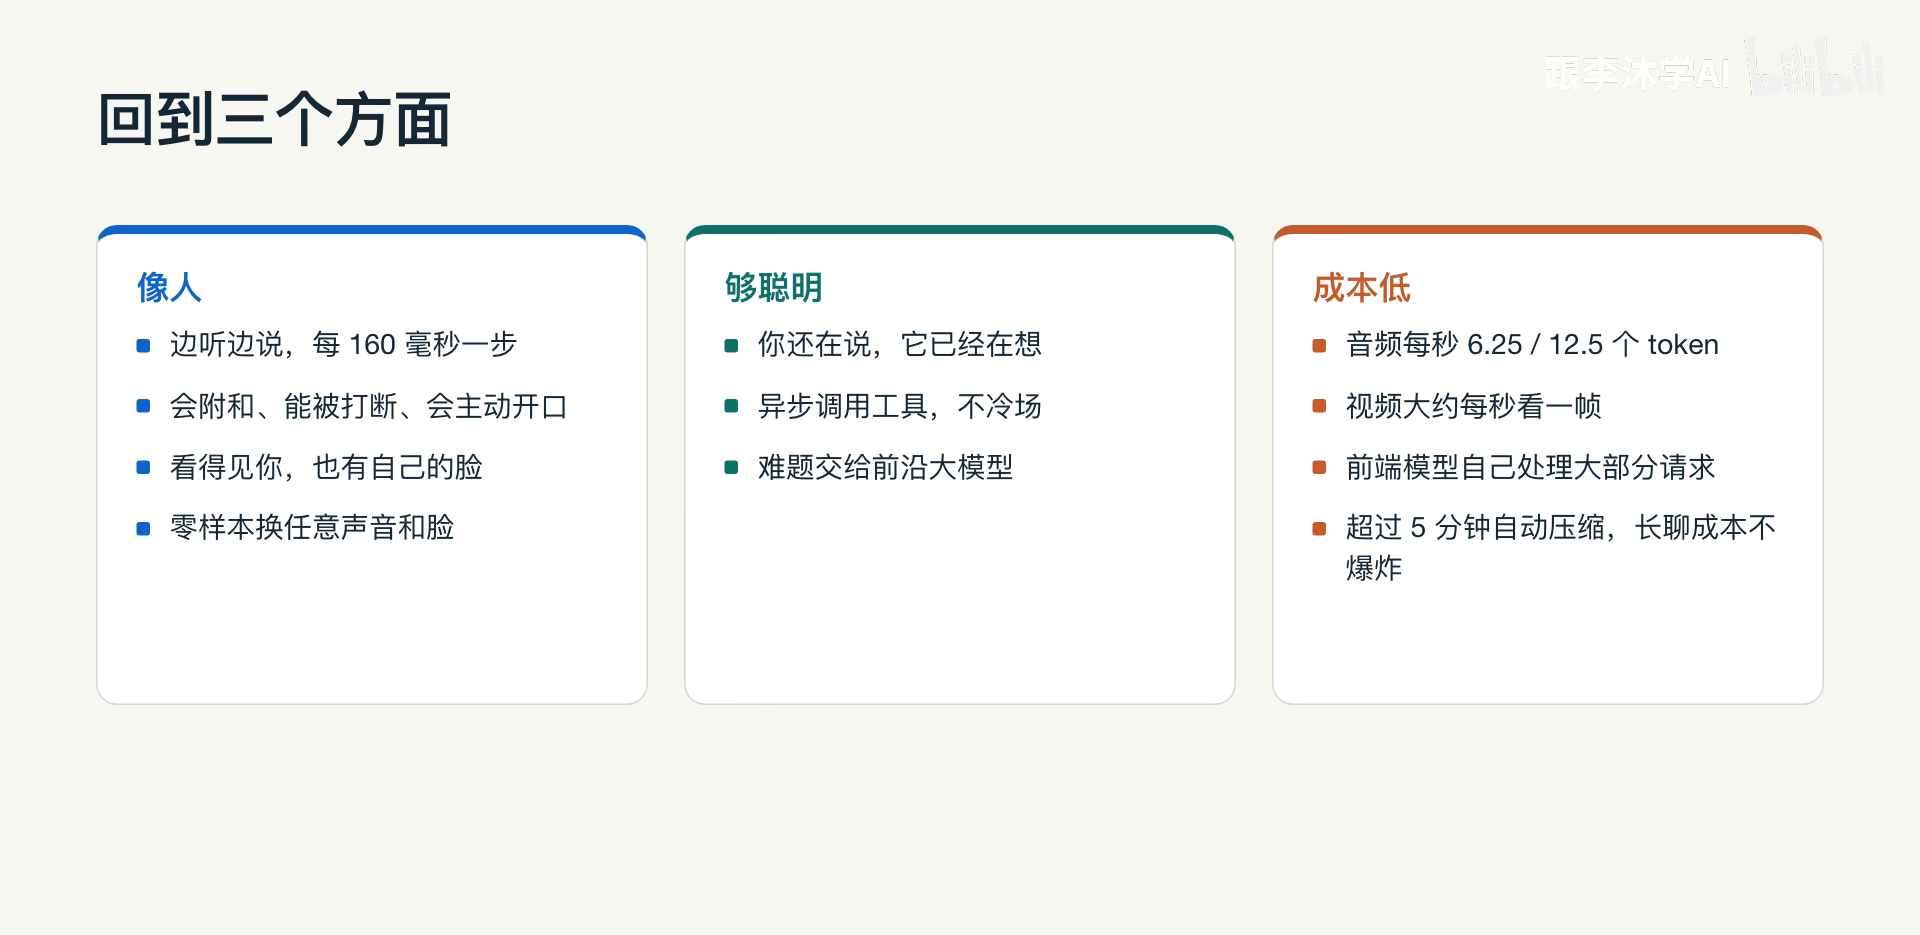
\includegraphics[width=0.95\textwidth]{figures/fig_27_summary_three_pillars.png}
\caption{回到三个方面：Higgs Realtime Duplex 围绕“像人”、“够聪明”与“成本低”三大核心目标所采取的全套架构与算法措施汇总\vtag}
\end{figure}
\srcnote{00:42:15--00:42:30}

\begin{figure}[H]
\centering
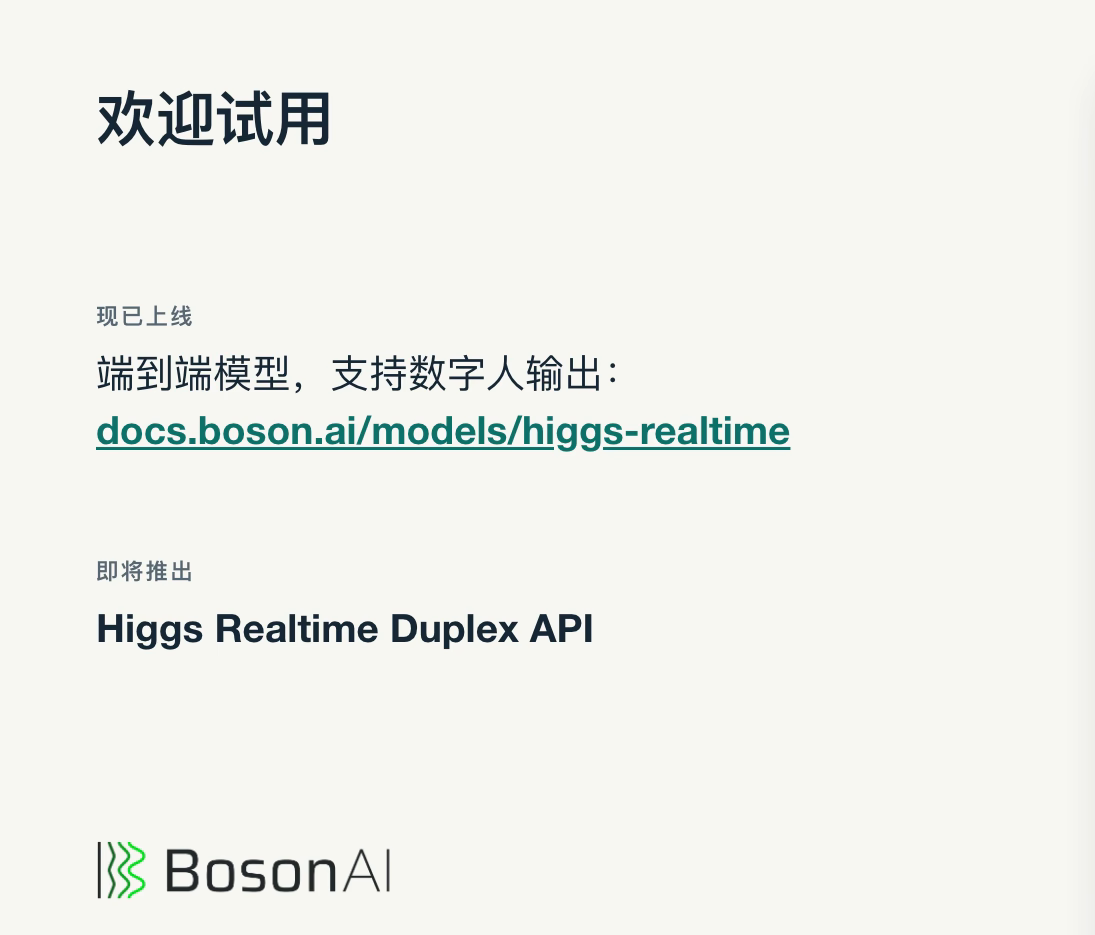
\includegraphics[width=0.74\textwidth]{figures/fig_28_closing_api_waitlist.png}
\caption{欢迎试用与展望：支持数字人输出的端到端模型 \texttt{Higgs Realtime} 已开放体验，全双工模型 \texttt{Higgs Realtime Duplex API} 即将上线\vtag}
\end{figure}
\srcnote{00:43:15--00:43:22}

\begin{importantbox}{全讲终极复盘：Higgs Realtime Duplex 是如何同时做到“像人、够聪明、成本低”的？}
\begin{enumerate}
    \item \textbf{如何做到“像人（Feels Human）”？}
    \begin{itemize}
        \item \textbf{边听边说，每 160毫秒预测一步}：彻底摒弃按轮次等待与外置 VAD，将响应与打断延迟压入 $0.1\text{--}0.2\,\mathrm{s}$ 真人生理区间；
        \item \textbf{能被打断、会附和、懂闭嘴}：通过 GRPO 与 RSI 仿真交互训练，学会边听边说“嗯哼”、遇插话即停、识别非对己旁话保持安静；
        \item \textbf{能看屏幕与摄像头，且自己有一张脸}：实时理解视觉流并同步渲染数字人表情，支持基于因果流匹配与因果 DiT 的**零样本换声音与换脸**。
    \end{itemize}
    \item \textbf{如何做到“够聪明（Smart）”？}
    \begin{itemize}
        \item \textbf{边说边在后台思考（Think）}：思维链跨越多个 160毫秒时间片持续延展，不阻塞语音输出；
        \item \textbf{异步调用工具（Call Tools）}：尽早发出工具请求，支持工具结果分阶段流式回流并先行播报初步结论；
        \item \textbf{按需委派给更大模型（Delegate）}：45B MoE 前端自主摆平绝大多数日常请求，遇到超难任务时异步交由后端前沿大模型攻关。
    \end{itemize}
    \item \textbf{如何做到“成本低（Costs Little）”？}
    \begin{itemize}
        \item \textbf{极致压缩音频流}：每 160毫秒仅用 $1$ 个输入音频 Token（$6.25\,\mathrm{tok/s}$）与 $2$ 个输出音频 Token（$12.5\,\mathrm{tok/s}$）；
        \item \textbf{稀疏视觉抽帧与紧凑面部表征}：每 6 个时间片（$0.96\,\mathrm{s}$）仅看 $1$ 帧视频，每步仅输出 $2$ 个面部 Latent；
        \item \textbf{前端分流 $+$ 超过 5分钟自动上下文压缩}：避免频繁唤醒昂贵后端模型，且只保留最近 5分钟完整多模态上下文（约 $13\mathrm{K}$ Token），更早历史压缩为纯文本，确保数小时长对话成本恒定可控。
    \end{itemize}
\end{enumerate}
\end{importantbox}

\subsection{本章小结}

本章全面解读了 \texttt{Higgs Realtime Duplex} 在七大权威基准上的评测表现，阐明了为何 45B MoE 前端模型能够匹敌甚至超越参数量大 6倍的 276B 模型，并围绕“像人、够聪明、成本低”黄金三角完成了全讲技术闭环总结。

\end{document}
